\documentclass[twoside,11pt]{article}
\usepackage[preprint]{dmlr2e}

% Allow long URLs (e.g. the artifact link) to break across lines.  Loading
% url after hyperref disables hyperlinked URLs but restores breakable ones.
\usepackage{url}
\makeatletter
\g@addto@macro\UrlBreaks{\do\a\do\b\do\c\do\d\do\e\do\f\do\g\do\h\do\i\do\j\do\k\do\l\do\m\do\n\do\o\do\p\do\q\do\r\do\s\do\t\do\u\do\v\do\w\do\x\do\y\do\z\do\A\do\B\do\C\do\D\do\E\do\F\do\G\do\H\do\I\do\J\do\K\do\L\do\M\do\N\do\O\do\P\do\Q\do\R\do\S\do\T\do\U\do\V\do\W\do\X\do\Y\do\Z\do\0\do\1\do\2\do\3\do\4\do\5\do\6\do\7\do\8\do\9}
\makeatother

\usepackage{float}
\usepackage{tikz}
\usepackage{amsmath}
\usepackage{booktabs}
\usepackage{array}
\usepackage{multirow}
\IfFileExists{microtype.sty}{\usepackage{microtype}}{} % optional polish; skip if not installed
\newcolumntype{L}[1]{>{\raggedright\arraybackslash}p{#1}}

\newcommand{\TTwoPatterns}{80}
\newcommand{\TTwoMean}{23.34}
\newcommand{\TTwoMedian}{19.4}
\newcommand{\TTwoSD}{19.8}
\newcommand{\TTwoPositive}{76}
\newcommand{\TTwoMin}{-3.9}
\newcommand{\TTwoMax}{75.7}
\newcommand{\TTwoSpearman}{-0.847}
\newcommand{\TTwoNGMedian}{0.714}
\newcommand{\TTwoBaseRSquared}{0.596}
\newcommand{\TTwoRelationRSquared}{0.691}
\newcommand{\TTwoLeaveMin}{20.91}
\newcommand{\TTwoLeaveMax}{24.64}
\newcommand{\TTwoBaseline}{0.612}
\newcommand{\TTwoEta}{0.494}
\newcommand{\TTwoInAbsentN}{50}
\newcommand{\TTwoInAbsentMean}{25.75}
\newcommand{\TTwoInPresentN}{30}
\newcommand{\TTwoInPresentMean}{19.32}
\newcommand{\TTwoInSpearman}{-0.149}
\newcommand{\TTwoInP}{0.188}
\newcommand{\TTwoDistinctOneN}{1}
\newcommand{\TTwoDistinctOneMean}{13.31}
\newcommand{\TTwoDistinctTwoN}{22}
\newcommand{\TTwoDistinctTwoMean}{22.90}
\newcommand{\TTwoDistinctThreeN}{57}
\newcommand{\TTwoDistinctThreeMean}{23.69}
\newcommand{\TTwoDistinctSpearman}{0.010}
\newcommand{\TTwoDistinctP}{0.931}

\newcommand{\TThreeFunctions}{40}
\newcommand{\TThreeBaseline}{0.768}
\newcommand{\TThreeMean}{1.83}
\newcommand{\TThreeSD}{0.97}
\newcommand{\TThreeMedian}{1.80}
\newcommand{\TThreeMin}{0.13}
\newcommand{\TThreeMax}{4.48}
\newcommand{\TThreePositive}{40}
\newcommand{\TThreeSpearman}{-0.727}
\newcommand{\TThreeNGMean}{0.077}
\newcommand{\TThreeNGMedian}{0.077}

\newcommand{\TNineMilpCases}{100}
\newcommand{\TNineDualCases}{100}
\newcommand{\TNineOddLower}{1.5}
\newcommand{\TNineOddUpper}{1.5}

\newcommand{\TTenM}{548}

\newcommand{\TSixCZeroAcc}{60.3}
\newcommand{\TSixCOneAcc}{82.8}
\newcommand{\TSixCTwoAcc}{64.0}
\newcommand{\TSixSemGain}{22.5}
\newcommand{\TSixDecoyGain}{3.7}
\newcommand{\TSixSemDecoyGain}{18.8}
\newcommand{\TSixSemLo}{16.8}
\newcommand{\TSixSemHi}{28.7}
\newcommand{\TSixDecoyLo}{1.3}
\newcommand{\TSixDecoyHi}{6.0}
\newcommand{\TSixSemDecoyLo}{13.2}
\newcommand{\TSixSemDecoyHi}{25.3}
\newcommand{\TSixSemSeedLo}{19.0}
\newcommand{\TSixSemSeedHi}{25.9}
\newcommand{\TSixDecoySeedLo}{0.0}
\newcommand{\TSixDecoySeedHi}{7.4}
\newcommand{\TSixSemDecoySeedLo}{13.0}
\newcommand{\TSixSemDecoySeedHi}{24.5}
\newcommand{\TSixProtocolHash}{0fb766ba884f}
\newcommand{\TSixTimingSeconds}{32.74}
\newcommand{\TSixPatterns}{40}



% The dmlr2e class hardcodes a "Reviewed on OpenReview: <link>" line in
% \@maketitle, intended for the camera-ready version.  A submission has no
% forum id yet, so the line is dropped here; at camera-ready, restore the
% class definition and set \openreview to the real forum URL.
\makeatletter
\def\@maketitle{\vbox{\hsize\textwidth
 \linewidth\hsize \vskip \beforetitskip
 {\begin{center} \Large\bf \@title \par \end{center}} \vskip \aftertitskip
 {\def\and{\unskip\enspace{\rm and}\enspace}%
  \def\addr{\small\it}%
  \def\email{\hfill\small\sc}%
  \def\name{\normalsize\bf}%
  \def\AND{\@endauthor\rm\hss \vskip \interauthorskip \@startauthor}
  \@startauthor \@author \@endauthor}
  \vskip \aftermaketitskip
  \if@preprint
  \else
  \noindent \@starteditor \@editor \@endeditor
  \vskip \aftermaketitskip
  \fi
}}
\makeatother

\setlength{\emergencystretch}{3em}

\ShortHeadings{Unseen Strings, Familiar Tasks}{Zhou} % TODO(authors): short author list
\firstpageno{1}

\begin{document}

\title{Unseen Strings, Familiar Tasks: Certified Semantic Exposure in
Procedural Reasoning Benchmarks}

% DMLR is single-blind: author names and affiliations are visible to reviewers.
\author{\name Zihan Zhou \email zihanzhou0725@gmail.com \\
       \addr School of Mathematical Sciences and Shanghai Center for
       Mathematical Sciences, Fudan University, 200433 Shanghai, China \\
       \addr Research Institute of Intelligent Complex Systems,
       Fudan University, 200433 Shanghai, China}

\maketitle

\begin{abstract}
Many reasoning benchmarks use a program to generate their tasks, and they
build the test set by holding out a representation: a parameter setting, a
rule string, or a program that never appeared in training.  We show that
such splits can fail silently, because different representations can
produce the same observable behavior.  Using tools that produce a proof for
every match, we audit three public protocols and find three distinct
failures.  In SLR-Bench, none of the 1,000 test rules repeats a training
string, yet we certify that at least 45.2\% are logically equivalent to a
training rule, with a checkable proof for every pair; the true overlap may
be higher.  In Tensor Logic, the split removes test edges from training but
breaks many of the paths that were meant to justify the test queries,
leaving between 484 and 1,000 of the 1,000 test queries with a matching
path still present in training.  In the Occam in-context-learning
benchmark, the generator keeps sampling from a small hidden pool of tasks:
at least two of the twenty evaluation tasks reappear in training, and the
true number may be as high as four.  We then asked whether seeing a task in
training actually changes what a model scores.  The answer depends on the
setting.  Across three Boolean in-context-learning tasks, removing exact
exposure changes mean accuracy by at most 0.09 points, even where exposure
reaches 93.44\%; a controlled six-architecture study finds a small gain
($+1.8$ points); and a preregistered experiment on the public CLUTRR
kinship benchmark, confirmed on fresh targets, finds a gain of $23.3$
points (95\% CI $[17.7, 29.2]$).  Our tools are simple in spirit: say what
``the same task'' means before measuring, grade how strong each piece of
evidence is, and report an interval instead of treating missing evidence as
no overlap.  Syntactic novelty is not semantic novelty, and exposure is not
exploitation; benchmark protocols should measure both.
\end{abstract}

\begin{keywords}
benchmark auditing, semantic novelty, data contamination, evaluation
methodology, preregistration
\end{keywords}

\section{Introduction}
\label{sec:introduction}

SLR-Bench is a published logical-reasoning benchmark whose test split is
built to be new: none of its 1,000 test rules repeats any of the 18,053
training rule strings \citep{helff2026slr}.  Under the benchmark's own
protocol, every test rule counts as an unseen task.  We show that this
guarantee does not hold.  Using a tool that rewrites rules into a standard
form and proves every match, we certify that at least 452 of the 1,000 test
rules---45.2\%---are logically equivalent to a training rule, and the true
overlap may be higher (Section~\ref{sec:public-audits},
Figure~\ref{fig:slr}).  The overlap is invisible to the split's own
criterion because the equivalent rules differ as strings: variables are
renamed, conditions reordered, redundant requirements dropped.

\begin{figure}[t]
\centering
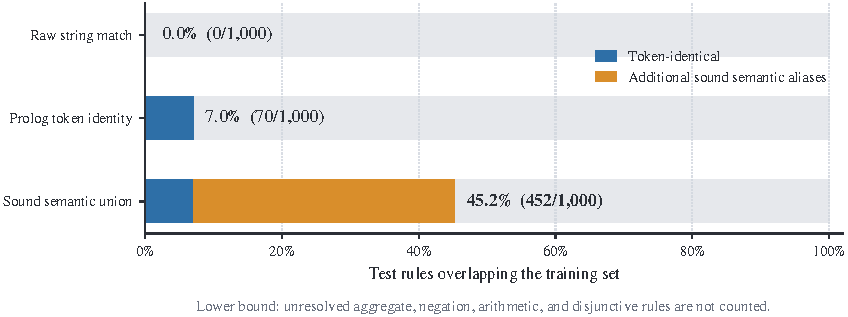
\includegraphics[width=0.94\textwidth]{figures/fig_slr_semantic_overlap.pdf}
\caption{SLR-Bench \texttt{v1-All}.  The split holds out rule strings, and
string matching finds zero overlap (left bar).  Token-level and
proof-producing semantic comparisons tell a different story, certifying a
45.2\% lower bound on train--test overlap.  Aggregate, negated, arithmetic,
and unresolved disjunctive rules are not counted, so the final bar is a
floor, not an estimate of total overlap.}
\label{fig:slr}
\end{figure}

Generated benchmarks are popular testbeds---for in-context function
learning \citep{garg2022what,akyurek2023what,bhattamishra2024understanding},
program induction \citep{reed2016neural,zaremba2014learning}, and
systematic generalization \citep{lake2018generalization}---because the
rules behind the data are known and new data can be sampled without manual
annotation.  But most of their splits hold out a \emph{representation}: a
parameter setting, a rule string, a program.  The evaluation claim,
meanwhile, is about a \emph{task}: the observable behavior that the
representation implements.  Because different representations can implement
the same behavior, a representation-level split cannot by itself certify a
task-level novelty claim.  We find that this gap opens in three distinct
ways across three public protocols: \emph{semantic aliases}, where
different rules induce the same logic (SLR-Bench); \emph{witness breakage},
where the mutation that hides test edges also deletes edges used by the
split's own witnesses (Tensor Logic: 379 of 1,000 designated test paths
survive, and between 484 and 1,000 of the 1,000 test queries still have a
matching path in training \citep{shah2026tensorlogic}); and
\emph{finite-space resampling}, where an online generator keeps drawing
from a small hidden task pool (in the Occam benchmark, at least two of
twenty evaluated tasks reappear in training, the true number may be four,
and at least 93.7\% of the 800,000 training episodes reuse an earlier
hidden task \citep{deora2025occam}).

Does such exposure actually change what models score?  The tempting answer
is yes, but it must be measured, and it is not uniform.  We ran three
controlled studies in which paired training runs differ only in whether the
target tasks are already seen during training.  Across three Boolean
in-context-learning tasks, removing exact exposure changes mean accuracy by
at most 0.09 percentage points, even where 93.44\% of the evaluation
functions appear in training.  A controlled six-architecture study finds a
small gain ($+1.8$ points).  A preregistered experiment on the public
CLUTRR kinship benchmark, confirmed on fresh targets, finds a gain of
$23.3$ points (95\% CI $[17.7, 29.2]$) \citep{sinha2019clutrr}.  Exposure
and exploitation are different things, and a credible benchmark audit must
report them separately.

Making such audits possible takes three simple tools.  An
\emph{observation contract} says, before any measurement, what ``the same
task'' means for a given claim.  An \emph{evidence grade} marks every
overlap finding as exact, a sound lower bound, estimated, or
unresolved---and unresolved items are never counted as novel.  A
\emph{certified exposure interval} turns an incomplete search for
equivalent items into explicit bounds $[L, U]$ instead of silently counting
them as zero.  An open toolkit checks every reported claim against its
declared unit, evidence grade, and source, and rebuilds the analyses in
this paper from saved result files.

\paragraph{Contributions.}
\begin{itemize}
\item \textbf{Findings.}  Certified audits of three public protocols: a
sound 45.2\% lower bound on semantic overlap for SLR-Bench despite zero
string-level overlap; witness breakage and endpoint exposure in $[484,
1000]/1000$ for Tensor Logic; and certified exposure of $[2, 4]/20$ tasks
under finite-space resampling in the Occam benchmark.
\item \textbf{Behavioral evidence.}  Three controlled studies that separate
exposure from exploitation, spanning a near-zero result (Boolean), a small
gain (six architectures), and a large gain (CLUTRR, preregistered,
confirmed on fresh targets).
\item \textbf{Instruments.}  Observation contracts, evidence grades, and
certified exposure intervals (Propositions 1 and 2), with an open,
schema-checked toolkit.
\item \textbf{Guidance.}  A short reporting standard for benchmark authors:
name the held-out object, grade the evidence, report the interval, and
measure behavior separately (Section~\ref{sec:recommendations}).
\end{itemize}

This is an evaluation-methodology study, not a new model or a general
procedure for program equivalence.  Its strongest conclusion is deliberately
bounded: training curricula that differ only in semantic exposure can
produce large differences in final accuracy, but exposure alone does not
reveal how a model obtained its prediction.

\section{What Counts as a New Task?}
\label{sec:measurement}

\begin{figure}[t]
\centering
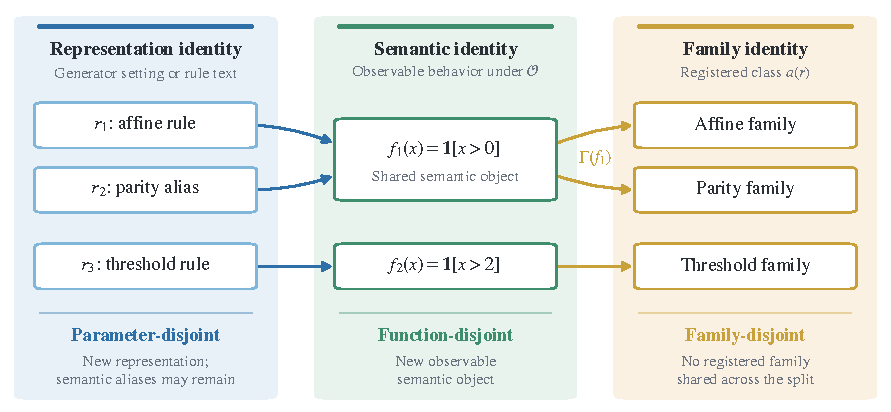
\includegraphics[width=0.98\textwidth]{figures/fig_semantic_identity_framework.pdf}
\caption{Three levels of novelty a split can claim.  A representation has a
registered family and, under an observation contract, induces a task---an
observable behavior.  Several representations, including ones from different
families, can induce the same task.  Holding out parameters, holding out
behaviors, and holding out families are therefore different promises.}
\label{fig:identity}
\end{figure}

\subsection{Representation, Task, and Family}

A generator parameter setting, a rule string, or a program is a
\emph{representation} $r$, drawn from a space $\mathcal R$.  An evaluation
claim, however, is rarely about the representation itself; it is about the
behavior the representation implements.  To make ``behavior'' precise, we
fix an \emph{observation contract} $\mathcal O$ before any measurement: a
written agreement on which inputs are allowed, which outputs are observed,
how termination, errors, and nondeterminism are treated, and nothing else.
Under a contract, each representation induces a semantic object through
\begin{equation}
q_{\mathcal O}:\mathcal R\rightarrow\mathcal F_{\mathcal O}.
\end{equation}
For the finite, deterministic, effect-free tasks studied here,
$\mathcal F_{\mathcal O}$ is simply the space of complete input--output
functions, and two representations are the \emph{same task} iff
$q_{\mathcal O}(r)=q_{\mathcal O}(r')$.  We do not assume that general
program equivalence is decidable; the contract only has to support the claim
at hand.

A representation also carries a family label $a(r)\in\mathcal G$, such as
``affine rule'' or ``parity rule.''  Families classify representations, not
tasks: one task can be implemented by representations from several families.
We write
\begin{equation}
\Gamma(f)=\{a(r):q_{\mathcal O}(r)=f\}.
\label{eq:family-relation}
\end{equation}
for the set of families that realize task $f$; the case $|\Gamma(f)|>1$ is
exactly the cross-family aliasing that our first behavioral study exploits
(Section~\ref{sec:internal-intervention}).

Figure~\ref{fig:identity} shows three things a split can hold out, and they
are not interchangeable.  \textbf{Parameter-disjoint} evaluation holds out
$r$ itself but may keep an alias $r'$ with
$q_{\mathcal O}(r')=q_{\mathcal O}(r)$.  \textbf{Function-disjoint}
evaluation holds out the behavior:
\begin{equation}
q_{\mathcal O}(\mathcal R_{\mathrm{train}})
\cap
q_{\mathcal O}(\mathcal R_{\mathrm{test}})
=\varnothing.
\label{eq:function-disjoint}
\end{equation}
\textbf{Family-disjoint} evaluation holds out the family label:
\begin{equation}
a(\mathcal R_{\mathrm{train}})
\cap
a(\mathcal R_{\mathrm{test}})
=\varnothing.
\label{eq:family-disjoint}
\end{equation}
Neither of the last two implies the other: two different tasks can share a
family, and two different families can implement the same task.

The \emph{semantic unit}---what counts as one task---must fit the claim and be
fixed before overlap is measured.  We ask for a prospective test: the claim
names what should stay fixed and what should vary, then supplies
\emph{must-match} pairs (items that should count as the same task) and
\emph{must-differ} pairs (items that should not).  A unit fails if it splits
a must-match pair or merges a must-differ pair; when several defensible units
pass and disagree, we report all of them rather than assert invariance.
Units differ by benchmark: a finite rule can be identified by its complete
output vector, a logic program by the relation it defines, CLUTRR by the
ordered relation composition plus the target relation rather than the story
string, and graph reasoning by endpoint-conditioned paths or relation
schemas.  Table~\ref{tab:summary} shows why this matters: Tensor Logic has
endpoint exposure $[484,1000]/1000$ but schema exposure $[999,1000]/1000$,
while SLR string identity gives zero overlap and the registered unit gives a
45.2\% sound lower bound; a single pooled ``contamination rate'' would erase
these distinctions.

\subsection{Evidence Grades}

Not every overlap finding is equally strong, and we keep the strength
attached to the finding.  A complete truth table or a provably injective
identifier gives an \emph{exact} test; a normalization that emits a proof for
every match gives a \emph{sound lower bound} (every collision it reports is
real, but items it cannot resolve may hide more); approximate execution
signatures give an \emph{estimate} and need an error analysis.  An unresolved
item is never evidence of novelty.  The grades describe identification
conditional on our machinery, not bugs inside it, so assurance is recorded
separately per audit: contract, source revisions and hashes, semantic-ID
implementation, soundness argument, validation coverage, known failure modes,
and qualitative residual risk (Table~\ref{tab:assurance};
Appendix~\ref{app:assurance}).

\subsection{Training-Budget Exposure}

Splits are not the only place novelty leaks: an online generator that draws
fresh episodes can still reuse tasks from a finite pool.  For a discrete
function distribution $p(f)$ and $N$ independent training draws, the
probability that an independent test function was seen during training is
\begin{equation}
P_{\mathrm{seen}}(N)
=
\sum_f p(f)\left[1-(1-p(f))^N\right].
\label{eq:coverage}
\end{equation}
The common shortcut $N/|\mathcal F|$ is valid only when sampling is uniform
and coverage is low.  A nonuniform sampler running a long stream makes
common functions almost certain to repeat while rare ones stay novel; the
Occam audit in Section~\ref{sec:public-audits} is exactly this failure.

\section{Auditing With Incomplete Evidence}
\label{sec:certification}

\subsection{The Audit Workflow}

Our audits follow four steps.  \textbf{First, declare the held-out object}:
text, parameters, complete functions, or families.  \textbf{Second, build
and grade a semantic signature}: exact maps when the space is finite,
proof-producing normalization when possible, explicitly estimated
signatures otherwise.  \textbf{Third, measure overlap under the actual
sampling budget}, including online training streams, not only the nominal
split.  \textbf{Fourth, separate validity from impact}: check whether the
protocol supports its novelty claim before asking whether the exposure
changed model behavior.

\subsection{When the Witness Search Is Incomplete, Report an Interval}

Equivalence search is often incomplete: some items carry a certificate,
others do not.  The temptation is to count the uncertified ones as novel.
That is wrong, and the fix is to report exactly what the certificates
imply.  Let $z_i$ indicate whether evaluation task $i$ occurred in
training.  A verified certificate on a group $G_j$ supplies
$\ell_j\leq\sum_{i\in G_j}z_i\leq u_j$.  For pairwise-disjoint certificate
groups and uncovered set $R$, Proposition~\ref{prop:certified} gives
\begin{equation}
\boxed{
\sum_j\ell_j
\leq C(E)
\leq |R|+\sum_j u_j
}.
\label{eq:certified-interval}
\end{equation}

\begin{proposition}[Certified exposure interval]
\label{prop:certified}
Under a frozen finite denominator, deterministic semantic identities, sound
group certificates, pairwise-disjoint groups, and no constraints on uncovered
items beyond binary membership, Equation~\ref{eq:certified-interval} contains
every exposure count consistent with the certificates, and both endpoints are
attained.
\end{proposition}

The proof is elementary, and we mean that as a feature: this is an accounting
device, not new mathematics.  The lower endpoint puts exactly $\ell_j$
exposed items in each group and none in $R$; the upper puts $u_j$ in each
group and all of $R$.  No tighter interval follows from those certificates
alone (proof, a grouped-seed corollary, and falsification tests are in
Appendix~\ref{app:certified}).  Operationally, an audit must report $[L,U]$,
and rows without witnesses stay out of the ``novel'' column.

When certificate groups overlap the closed form no longer applies; the
toolkit either solves the binary program exactly by mixed-integer linear
programming or returns a linear-programming outer interval with independently
checkable dual certificates (Appendix~\ref{tmlrs:app:overlap}).

A downstream question asks how well the truly novel subset could be doing
among unresolved items with observed scores;
Proposition~\ref{tmlrs:prop:novelty} gives the sharp answer.

\begin{proposition}[Novelty-conditioned score interval]
\label{tmlrs:prop:novelty}
Let $\mathcal{R}$ be $M$ unresolved items with observed scores
$y_i\in[0,1]$, sorted as
$y_{(1)}\leq\cdots\leq y_{(M)}$, and suppose at most $U<M$ of them are
exposed.  Then the mean score on the truly novel items lies in
\[
\left[
\frac{1}{M-U}\sum_{k=1}^{M-U}y_{(k)},\
\frac{1}{M-U}\sum_{k=U+1}^{M}y_{(k)}
\right],
\]
both endpoints are attained by some admissible novel set, and the interval
widens monotonically in $U$.
\end{proposition}

This is a trimming bound in the sense of \citet{lee2009training} and
\citet{horowitz1995identification}: without a nontrivial upper bound on
exposure, any nonempty subset could be the novel one and the interval is
$[\min_i y_i,\max_i y_i]$ (sensitivity to $U$ and proof in
Appendix~\ref{tmlrs:app:novelty-proof}).  The bound isolates witness
incompleteness only: it assumes correct sources, semantic IDs, and
certificate implementations, and does not absorb machinery failures, so it is
read together with the assurance record.

For compactness, the summary table abbreviates confidence interval (CI) and
in-context learning (ICL).

\begin{table}[t]
\caption{Cross-benchmark evidence summary.  Semantic units differ by row and
must not be pooled into a prevalence estimate.}
\label{tab:summary}
\centering
\small
\setlength{\tabcolsep}{3.5pt}
\begin{tabular}{L{0.85in}L{1.02in}L{1.70in}L{1.95in}}
\toprule
Case & Nominal holdout & Measured semantic exposure &
Behavioral evidence \\
\midrule
Exact-alias intervention &
Cross-family representation &
Complementary exposure of 40 exact functions &
$+1.832$ pp macro, 95\% CI $[1.470,2.189]$ \\
Boolean ICL &
Fresh function draw &
0.81--93.44\% exact exposure &
$-0.06$ to $+0.09$ pp; below preregistered threshold \\
CLUTRR &
Disjoint source stories and permutations &
Randomized exposure of relation-composition patterns &
V4: $+23.339$ pp, 95\% CI $[17.750,29.226]$ \\
SLR-Bench &
Raw rule string &
$\geq45.2\%$ sound logical overlap &
Identification stopped before outcome fitting \\
Tensor Logic &
Direct-edge removal &
$[484,1000]/1000$ endpoint; $[999,1000]/1000$ schema &
No reproducible checkpoint or per-item outputs \\
Occam Markov &
Unseen transition task &
$[2,4]/20$ exact tasks per main experiment &
Aggregate plots only; regression scope unavailable \\
\bottomrule
\end{tabular}
\end{table}

\section{Does Exposure Change Behavior?  Two Controlled Studies}
\label{sec:behavior}

Knowing that a test task was exposed does not say whether the exposure
helped.  We therefore ran controlled studies with frozen endpoints and
paired training runs that differ only in which target tasks are exposed.
This section reports two of them, with opposite outcomes: a small positive
gain in a controlled six-architecture study, and a near-zero result in a
Boolean in-context-learning task despite almost complete exposure.
Section~\ref{sec:clutrr-external-validation} reports the third, a large
gain on the public CLUTRR benchmark.  The studies share a design idea but
deliberately no pooled effect estimate.

\subsection{Study 1: Exact Aliases in a Controlled Generator}
\label{sec:internal-intervention}

Our finite rule generator has 560 parameter identities but only 518
complete functions: exactly 40 functions are implemented twice, once by an
affine rule and once by a parity rule.  This is the cleanest possible
testbed for aliasing.  We pair the two identities of each aliased function
($f_{1,b}$ with $f_{11,b}$ for each intercept $b\in\{0,\ldots,19\}$).  For
each model seed, a frozen SHA-256 bit assigns one member of every pair to
Arm~A and the other to Arm~B, so every target is exposed in exactly one arm
and unexposed in the other.  Both arms share 478 common base functions,
equal family counts, and 20,000 paired episodes; initialization, episode
order, and optimizer schedule are identical.

We train six architectures---Deep Sets \citep{zaheer2017deep}, Relation
Network \citep{sung2018relation}, Set Transformer \citep{lee2019set},
modern Hopfield retrieval \citep{ramsauer2021hopfield}, Perceiver
\citep{jaegle2021perceiver}, and Transformer
\citep{vaswani2017attention}---with five seeds and two arms, giving 60 fixed
epoch-60 runs, all evaluated on the same 10,000 episodes.  Let $\mathbf
Z_s^A\in\{0,1\}^{40}$ record the target-exposure assignments in Arm~A and
$\mathbf Z_s^B=\mathbf 1-\mathbf Z_s^A$; for target $f$, $\mathbf
Z_{s,f}^{(1)}$ is whichever complete arm vector exposes $f$.  Writing
$A(m,s,f;\mathbf z)$ for accuracy under a complete assignment, the primary
estimand is the average exposed-minus-unexposed difference
\begin{equation}
\tau_{\mathrm{macro}}
=
\frac{1}{6}\sum_m
\frac{100}{5\cdot40}\sum_{s,f}
\left[
A(m,s,f;\mathbf Z_{s,f}^{(1)})
-A(m,s,f;\mathbf Z_{s,f}^{(0)})
\right].
\end{equation}
Because randomization flips complete curricula rather than one target at a
time, cross-target transfer or interference is part of the identified
contrast, not a separate quantity.

\begin{table}[t]
\caption{Preregistered exact-exposure intervention.  Accuracy is percent.
Architecture intervals use Bonferroni simultaneous 99.1667\% confidence; the
equal-architecture macro uses the registered hierarchical 95\% bootstrap.}
\label{tab:internal-models}
\centering
\small
\setlength{\tabcolsep}{5pt}
\begin{tabular}{lrrrl}
\toprule
Architecture & Exposed & Unexposed & Effect (pp) &
Simultaneous CI \\
\midrule
Deep Sets & 59.60 & 53.49 & +6.110 & $[4.349,7.849]$ \\
Relation Network & 88.34 & 87.34 & +0.996 & $[0.229,1.749]$ \\
Set Transformer & 77.80 & 76.76 & +1.042 & $[-0.105,2.247]$ \\
Modern Hopfield & 88.66 & 88.00 & +0.658 & $[-0.192,1.447]$ \\
Perceiver & 74.41 & 73.12 & +1.284 & $[-0.042,2.525]$ \\
Transformer & 82.94 & 82.04 & +0.902 & $[-0.137,1.870]$ \\
\midrule
Architecture macro & 78.63 & 76.79 & +1.832 &
$[1.470,2.189]$ (95\%) \\
\bottomrule
\end{tabular}
\end{table}

The preregistered macro criterion passes: the effect is $+1.832$ points,
its 95\% lower confidence endpoint is positive, and all six architecture
estimates are positive.  Only Deep Sets meets the stricter per-architecture
rule (at least one point with its simultaneous interval excluding zero).
Cross entropy and Brier score improve by $0.0786$ and $0.0267$.  So exact
cross-family aliases do produce a measurable endpoint effect here---small,
but reliable.  The design identifies a curriculum-level effect for these
architectures and this budget; it says nothing about any internal
memorization mechanism.

\subsection{Study 2: A Near-Zero Contrast at High Exposure}
\label{sec:boolean}

The released Boolean in-context-learning generators
\citep{bhattamishra2024understanding} give the opposite outcome, and a
useful counterexample to the shortcut ``overlap implies a performance
gain.''  Here the semantic IDs are exact: signed-literal vectors for
Conjunction-28, active-variable masks for Majority-28, and four-element
literal subsets for Sparse Disjunction-50.  At the frozen 640,000-episode
training budget, 0.81\%, 8.88\%, and 93.44\% of the evaluation functions
already occur in the original training streams.

Before any training, we froze 1,280 evaluation functions per task, three
original streams, and paired \emph{strict} streams that replace only the
training slots colliding with an evaluation semantic ID.  The released
six-layer Transformer is trained for 20,000 fixed steps with three seeds
under both streams.  The endpoint is mean sign accuracy at prompt positions
20--39, with \(\Delta_{\rm pp}=100(A_{\rm Original}-A_{\rm Strict})\).

\begin{table}[t]
\caption{Boolean exposure and registered behavioral effects.  Hierarchical
intervals resample model seeds and semantic-ID clusters.}
\label{tab:boolean-main}
\centering
\small
\begin{tabular}{lrrl}
\toprule
Task & Exposure (\%) & Mean effect (pp) & 95\% CI \\
\midrule
Conjunction & 0.81 & $-0.013$ & $[-0.092,0.044]$ \\
Majority & 8.88 & $-0.064$ & $[-0.199,0.078]$ \\
Sparse Disjunction & 93.44 & $+0.092$ & $[-0.060,0.282]$ \\
\bottomrule
\end{tabular}
\end{table}

No task reaches the frozen two-point threshold, and no task has three
positive seed deltas, so neither preregistered success criterion is met and
the planned seed and model expansion was not run.  Even at 93.44\% exact
exposure, the effect stays within a tenth of a point.  The result is bounded
to this model, budget, and released task definitions; it does not show that
exposure can never matter.  Together with the small positive result above,
it shows why exposure prevalence and behavioral effect are separate
measurements.

\section{Study 3: A Large Preregistered Gain on CLUTRR}
\label{sec:clutrr-external-validation}

The first two studies use synthetic tasks with small models; neither
involves a public, natural-language-like reasoning benchmark.  We therefore
ran a controlled experiment on CLUTRR \cite{sinha2019clutrr}, a public
benchmark of kinship reasoning from generated text.  The question is
narrow: \emph{does training on one set of surface realizations of a
relation pattern improve accuracy on fresh realizations of the same
semantic pattern?}  We report a preregistered pilot (V3) and a
preregistered confirmation on disjoint targets (V4).  The two studies are
never pooled.

\subsection{Task, Unit, and Design}

We freeze CLUTRR Task~1 at relation length three, without distractor facts.
Each example contains a three-edge kinship chain and a query relation drawn
from 23 classes, and entity names are canonicalized by order of appearance.
The semantic identity of an example is the ordered tuple of the target
relation and the three edge relations; sentence order is a surface property
and is not part of the identity.

For every three-sentence source story, we enumerate all six sentence
permutations and group them under one source-group identifier.  A target
pattern is eligible only when it has at least 45 complete source groups.
Its evaluation set contains 200 rows from the first 34 sorted groups (all
six permutations of groups 0--32 and two permutations of group~33); its
training exposure contains 64 rows from the next 11 groups (all six
permutations of groups 34--43 and four of group~44).  Evaluation and
exposure therefore share no source group.

Targets are paired only within the same output relation.  For each model
seed, a frozen SHA-256 bit exposes one pair member in Arm~A and the other
in Arm~B.  Both arms share a 22,720-row base with no target semantics and
append 1,280 target-exposure rows, giving 24,000 training rows per run with
identical label counts.  Initialization, all 30 epoch permutations, tensor
shapes, and dropout RNG trajectories are paired across complementary runs.
The model is a fixed four-layer byte-level Transformer (model dimension
128, four attention heads, feed-forward dimension 512, dropout 0.1),
trained with AdamW at batch size 128 and learning rate $3\times10^{-4}$
under deterministic float32 CPU execution, and evaluated at the fixed
epoch-30 checkpoint after 5,640 updates.  There is no validation selection
or early stopping, and the evaluation manifest is identical across arms
within a block.

\subsection{Estimand and Inference}

For seed $s$, let $\mathbf Z_s^A\in\{0,1\}^{F}$ record which target patterns
are exposed in Arm~A, with
$\mathbf Z_s^B=\mathbf 1-\mathbf Z_s^A$.  For target $f$,
$\mathbf Z_{s,f}^{(1)}$ denotes whichever complete arm assignment exposes
$f$, and $\mathbf Z_{s,f}^{(0)}$ is the complementary assignment.  Let
$A_{s,f}(\mathbf z)$ be row-weighted accuracy under complete assignment
$\mathbf z$.  For $S$ frozen seeds and $F$ frozen targets, the sole primary
estimand is
\begin{equation}
\tau
=
\frac{100}{SF}
\sum_{s=1}^{S}\sum_{f=1}^{F}
\left[
A_{s,f}(\mathbf Z_{s,f}^{(1)})
-A_{s,f}(\mathbf Z_{s,f}^{(0)})
\right]
\quad\text{percentage points}.
\label{eq:clutrr-exposure-estimand}
\end{equation}
As in Study~1, this is the average contrast between two complete
complementary curricula; it includes cross-pattern transfer rather than
isolating one pattern's direct effect.

The 95\% interval uses 20,000 hierarchical percentile-bootstrap replicates
that resample model seeds, complete same-label target pairs, and source
groups within each selected pair member, with source-group draws shared
between exposed and unexposed predictions.  The point estimand is the
finite average over the eight frozen seeds and 80 frozen V4 targets.  The
interval treats the observed seeds, pairs, and within-target source groups
as exchangeable draws from their empirical distributions, conditional on
this model, task, eligibility filter, exposure dose, and budget; because
target selection and group allocation were deterministic, it is not
design-based inference for all eligible CLUTRR patterns, stories, relation
lengths, or architectures.  As a post-hoc sensitivity check, an
intercept-only CR1 cluster-robust estimator clusters the 640 seed-pattern
effects by seed and by complete target pair; the two-way cluster standard
error is 2.6187 points, and a conservative $t_7$ interval is
$[17.1469,29.5313]$.  This check does not replace the registered bootstrap
or alter the decision rule.

\begin{table}[t]
\caption{CLUTRR exposure interventions.  V3 and V4 use disjoint target
semantic patterns and are not pooled.}
\label{tab:clutrr-external-validation}
\centering
\scriptsize
\setlength{\tabcolsep}{3pt}
\begin{tabular}{lrrrrL{1.55in}}
\toprule
Study & Pairs & Targets & Runs & Effect (pp) &
95\% CI; registered outcome \\
\midrule
V3 pilot & 20 & 40 & 16 & $+15.338$ &
$[9.877,21.369]$; precision criterion not met \\
V4 confirm. & 40 & 80 & 32 & $+23.339$ &
$[17.750,29.226]$; directional criterion met \\
\bottomrule
\end{tabular}
\end{table}

\subsection{V3: A Positive but Imprecise Pilot}

V3 froze 20 same-label pattern pairs, eight model seeds, and two arms (16
runs).  Its preregistration allowed a positive, negative, or equivalence
conclusion only if the 95\% interval was at most two points wide.  The
observed effect was $+15.3375$ points with interval $[9.8769,21.3693]$:
positive throughout, but 11.4924 points wide, so the registered outcome is
``positive but imprecise.''  We keep that label rather than relabeling the
pilot after seeing a large estimate.  A post-hoc variance diagnosis
attributes 94.40\% of the bootstrap variance to target-pair resampling, and
a calibrated projection shows that the two-point precision target would
need at least 634 independent pairs while only 139 V3-disjoint eligible
pairs remained.  The strict-precision route was closed, and V3 served only
as a pilot for designing V4.

\subsection{V4: Preregistered Confirmation on Fresh Targets}

Before any V4 training outcome existed, we froze a directional design based
only on V3: a design effect of $7.66875$ points (the smaller of half the V3
point estimate and its lower interval endpoint) and a 100,000-draw Monte
Carlo power analysis over one to four 20-pair blocks.  One block had power
0.7440 and failed; two blocks had power 0.9583 with a 95\% Wilson lower
bound of 0.9570 and were selected.  All 80 V4 targets are semantically
disjoint from the V3 targets, and the success criterion required
$\tau\geq1$ point with the two-sided 95\% interval above zero.

All 32 runs reached the fixed checkpoint and passed post-training integrity
checks: finite model and optimizer state, frozen epoch orders, four-way
paired RNG trajectories, prediction ordering, separate-code-path metric
recomputation, and artifact hashes.  The confirmatory effect is $+23.3391$
points, 95\% CI $[17.7498,29.2257]$: the criterion is met.  Both block
estimates were positive ($+25.0109$ and $+21.6672$ points), as were all
eight seed estimates and all 40 pair estimates; 76 of 80 target patterns
were positive.  These sign counts are descriptive and were not additional
tests.  The secondary proper losses move in the same direction
(exposed-minus-unexposed cross entropy $-1.4938$, multiclass Brier score
$-0.4224$, ECE-15 $-0.2018$); they were registered as descriptive and
cannot alter the accuracy-based primary conclusion.

\subsection{Why Do the Effects Differ?}
\label{sec:why-effects-differ}

The three studies span a near-zero Boolean result, a $+1.8$-point internal
gain, and a $+23.3$-point CLUTRR gain.  We treat this range as the main
behavioral finding, not as noise to average away.  A plausible reading,
which we flag as post hoc: exposure buys little when the model already
executes a short reusable rule (the Boolean tasks, where the released
Transformer scores about 93\% on Conjunction and 78--83\% on Majority and
Sparse Disjunction even without exposure); it buys more where withheld
compositions must be inferred from a limited set of neighbors (CLUTRR
trains a small byte-level model from scratch at one relation length and a
modest budget, a regime in which large seen-versus-unseen gaps are
expected).  A large CLUTRR gap is therefore not surprising in itself.  What
the framework adds is that the gap is attributed to a certified semantic
exposure difference under a preregistered, target-disjoint design, rather
than to a surface-form split that may or may not change semantic exposure.
The practical implication is direct: whether semantic exposure matters is
an empirical property of a model, budget, and task family, so a benchmark
that claims semantic novelty should measure the exposure contrast rather
than assume either a large or a negligible effect.  Figure~\ref{fig:forest}
places the three effects on one axis.

\begin{figure}[t]
\centering
\scriptsize
\definecolor{fblue}{RGB}{46,111,167}
\definecolor{forange}{RGB}{217,142,43}
\definecolor{fgray}{RGB}{107,114,128}
\definecolor{fdark}{RGB}{75,85,99}
\definecolor{fink}{RGB}{43,47,54}
\begin{tikzpicture}[x=1cm, y=0.62cm, font=\scriptsize]
  % study bands: near-zero studies vs large-effect studies
  \fill[fdark!14] (0.8,-0.35) rectangle (9.15,3.55);
  \fill[forange!24] (0.8,3.55) rectangle (9.15,5.45);
  \draw[fdark!35, line width=0.4pt] (0.8,3.55) -- (9.15,3.55);
  % vertical grid
  \foreach \x in {0.8,1.6,2.4,3.2,3.9455,6.4005,8.8555} {
    \draw[gray!25, densely dotted] (\x,0) -- (\x,5);
  }
  % zero line
  \draw[fink, line width=0.5pt] (0.8,-0.35) -- (0.8,5.55);
  % confidence intervals and point estimates
  \draw[fdark, line width=1pt] (0.7264,0) -- (0.8352,0);
  \fill[fdark] (0.7896,0) circle (2pt);
  \draw[fdark, line width=1pt] (0.6408,1) -- (0.8624,1);
  \fill[fdark] (0.7488,1) circle (2pt);
  \draw[fdark, line width=1pt] (0.752,2) -- (1.0256,2);
  \fill[fdark] (0.8736,2) circle (2pt);
  \draw[fblue, line width=1pt] (1.976,3) -- (2.5512,3);
  \fill[fblue] (2.2656,3) circle (2pt);
  \draw[forange!55, line width=1pt] (3.9153,4) -- (6.7367,4);
  \draw[forange!55, line width=0.9pt, fill=white]
    (5.2559,4) circle (2pt);
  \draw[forange, line width=1pt] (5.8481,5) -- (8.6654,5);
  \fill[forange] (7.2203,5) circle (2pt);
  % broken horizontal axis
  \draw[fink, line width=0.5pt] (-0.05,-0.55) -- (3.2,-0.55);
  \draw[fink, line width=0.5pt] (3.7,-0.55) -- (9.15,-0.55);
  \draw[fink, line width=0.5pt] (3.28,-0.62) -- (3.42,-0.48);
  \draw[fink, line width=0.5pt] (3.55,-0.62) -- (3.69,-0.48);
  \foreach \x/\v in {0.8/0,1.6/1,2.4/2,3.2/3} {
    \draw[fink, line width=0.5pt] (\x,-0.55) -- (\x,-0.65)
      node[below] {$\v$};
  }
  \foreach \x/\v in {3.9455/10,6.4005/20,8.8555/30} {
    \draw[fink, line width=0.5pt] (\x,-0.55) -- (\x,-0.65)
      node[below] {$\v$};
  }
  \node[below=0.92cm] at (4.6,-0.55)
    {Exposure effect, exposed minus unexposed (percentage points)};
  % row labels
  \node[anchor=east] at (-0.12,0) {Conjunction};
  \node[anchor=east] at (-0.12,1) {Majority};
  \node[anchor=east] at (-0.12,2) {Sparse Disjunction};
  \node[anchor=east] at (-0.12,3) {Internal (6 architectures)};
  \node[anchor=east] at (-0.12,4) {CLUTRR V3 (pilot)};
  \node[anchor=east] at (-0.12,5) {CLUTRR V4 (confirmatory)};
  % values
  \node[anchor=west] at (9.25,0) {$-0.01\ [-0.09,0.04]$};
  \node[anchor=west] at (9.25,1) {$-0.06\ [-0.20,0.08]$};
  \node[anchor=west] at (9.25,2) {$+0.09\ [-0.06,0.28]$};
  \node[anchor=west] at (9.25,3) {$+1.8\ [1.5,2.2]$};
  \node[anchor=west] at (9.25,4) {$+15.3\ [9.9,21.4]$};
  \node[anchor=west] at (9.25,5) {$+23.3\ [17.7,29.2]$};
  % legend, below the axis title
  \node at (1.30,-3.0) {\textcolor{fdark}{$\bullet$}~Boolean ICL};
  \node at (4.05,-3.0) {\textcolor{fblue}{$\bullet$}~Internal study};
  \node at (6.95,-3.0) {\textcolor{forange}{$\bullet$}~CLUTRR};
\end{tikzpicture}
\caption{Exposure effects across the three controlled studies: exposed
minus unexposed accuracy, in percentage points, with 95\% confidence
intervals.  Colors group the studies: dark gray for the Boolean tasks, blue
for the internal six-architecture study, orange for CLUTRR.  Filled circles
are confirmatory estimates; the open circle is the CLUTRR V3 pilot, which
was positive but did not meet its preregistered two-point precision
criterion.  The horizontal axis is broken between 3 and 9 points because
the Boolean and internal effects sit at zero while the CLUTRR effects are
an order of magnitude larger; that gap is the finding, not a scaling
artifact.}
\label{fig:forest}
\end{figure}

Within CLUTRR, pattern-level effects range from \TTwoMin{} to
\TTwoMax{}~pp and are strongly predicted by the unexposed baseline
(Spearman $\rho=\TTwoSpearman{}$); the median normalized gain is
\TTwoNGMedian{} (Appendix~\ref{tmlrs:app:clutrr-heterogeneity}).
The same headroom pattern holds in the internal finite-function study
(Spearman $\rho=\TThreeSpearman{}$), where the model is near ceiling and
the median normalized gain is only \TThreeNGMedian{}
(Appendix~\ref{tmlrs:app:internal-heterogeneity}).
In a further exploratory (not preregistered) CLUTRR experiment,
same-semantic exposure changes accuracy by \TSixSemGain{}~pp, versus
\TSixDecoyGain{}~pp for relation-matched decoys sharing at least two edge
types; the direct contrast is \TSixSemDecoyGain{}~pp
(95\% CI [\TSixSemDecoyLo{}, \TSixSemDecoyHi{}];
Appendix~\ref{tmlrs:app:semantic-surface}).
The decoy contrast has a positive pattern-cluster interval, but its
four-seed interval includes zero; a zero decoy effect is not excluded
by the seed-level analysis.

\begin{figure}[t]
\centering
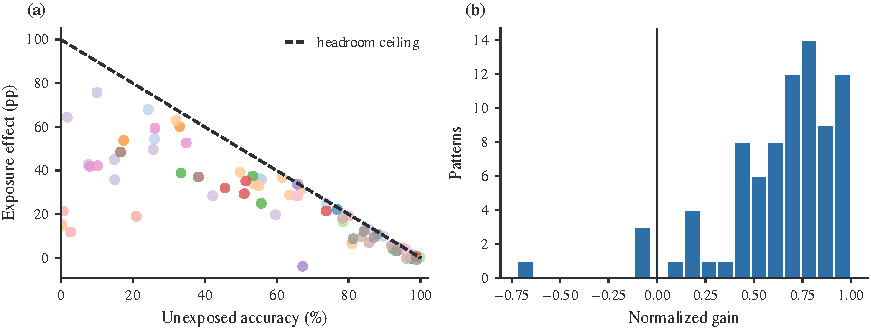
\includegraphics[width=0.98\textwidth]{figures/tmlrs_clutrr_heterogeneity.pdf}
\caption{Exploratory (not preregistered) heterogeneity across the
\TTwoPatterns{} CLUTRR V4 semantic patterns.  In (a), points are colored
by target relation and the dashed line marks the headroom ceiling;
effects are largest when unexposed accuracy leaves more headroom.
Normalized gain (b) remains high for most patterns.}
\label{tmlrs:fig:clutrr-heterogeneity}
\end{figure}

\subsection{What the CLUTRR Result Does and Does Not Say}

The experiment identifies an endpoint effect of randomized complementary
curricula in the frozen CLUTRR setting: the curriculum that exposes a focal
relation composition yields higher focal-pattern accuracy than its paired
alternative, on different source groups and sentence permutations.  This is
a behavioral consequence beyond exact-string reuse, and it supplies the
public-benchmark behavior that the structural audits lack.  It does not
isolate the direct effect of one pattern's exposure from transfer among the
other patterns whose assignments also reverse.

The claim remains deliberately bounded: one CLUTRR task, one relation
length, one architecture, one exposure dose, one optimization budget.  The
result does not show that every form of semantic overlap improves accuracy,
that the model stores a literal lookup table, or that the same effect holds
for unseen relation lengths, family-disjoint reasoning, other
architectures, or natural text.  The near-zero Boolean result stands as a
counterexample to the universal shortcut ``overlap implies memorization.''
The combined evidence supports the weaker and more useful conclusion:
curricula that differ in semantic exposure can have a large behavioral
effect, so benchmark novelty and behavioral exploitation must be measured
separately.


\section{Auditing Three Public Protocols}
\label{sec:public-audits}

The controlled studies estimate behavior when retraining is feasible.  The
structural audits here answer the prior question: does a released protocol
support the semantic novelty it claims?  Each case keeps its own semantic
namespace, witness completeness, and claim boundary; we do not pool them
into a prevalence estimate.

\subsection{SLR-Bench: String Novelty Masks Logical Overlap}
\label{sec:slr}

SLR-Bench contains 20 curriculum levels generated by an automated
logical-reasoning framework \citep{helff2026slr}; its released
\texttt{v1-All} split has 18,053 training rows and 1,000 test rows, and no
test rule string appears verbatim in training.  String exclusion, however,
is not logical novelty.  Tokenizing Prolog while ignoring whitespace
already finds 70 test rules identical to a training rule.  For flat
positive rules, we additionally canonicalize variable names and condition
order, drop duplicate existential profiles, and drop existential conditions
that a stronger profile already entails.  This proves 382 further
train--test equivalences.  The two sets are disjoint, so
\begin{equation}
\frac{70+382}{1000}=45.2\%
\end{equation}
is a sound lower bound (Figure~\ref{fig:slr}).

The mechanism is ordinary logic, not fuzzy similarity.  Without variable
inequality,
\begin{equation}
\exists x\,P(x)\land\exists y\,P(y)
\equiv
\exists x\,P(x),
\end{equation}
because both variables may bind to the same object.  Likewise, a weaker
existential condition is redundant when a stronger profile entails it.
Every reported pair comes with a train rule, a test rule, and the canonical
witness, so the 45.2\% figure can be checked pair by pair rather than
believed.

We do not infer model impact from the released per-item prediction
artifact: although it aligns with all 1,000 test IDs and reference rules,
its Basic-tier accuracy does not reproduce the paper's reported aggregate.
A preregistered adjusted overlap--correctness analysis also stopped before
fitting, because the output is not tied to a reproducible checkpoint and
exact curriculum-level common support retains only 352/452 witnessed rows
(77.88\%), below the frozen 80\% threshold.  SLR therefore supports the
structural lower bound, not a performance-inflation estimate.

For the \TTenM{} unresolved SLR-Bench items, an exploratory
(not preregistered) sensitivity analysis leaves the correct fraction $p$
unspecified: Proposition~\ref{tmlrs:prop:novelty} gives
$[\max(0,pM-U),\min(pM,M-U)]/(M-U)$ for an assumed exposure upper bound
$U<M$.  Appendix~\ref{tmlrs:app:novelty-proof} shows how wide the interval
can get, without using the released prediction artifact or estimating model
performance.

\subsection{Two More Failure Modes: Broken Witnesses and Resampled Pools}
\label{sec:tl-occam}

\textbf{Witness breakage (Tensor Logic).}  The compositional split of
\citet{shah2026tensorlogic} selects two-hop test paths and then removes the
1,000 direct test edges from training.  Edge removal works; path removal
does not.  Because the removal is global, it can delete an edge that another
selected path relies on, and only 379 of the 1,000 designated test paths
survive.  Allowing alternative intermediate entities, 484 of 1,000 queries
retain an endpoint-level witness in training, while the ordered
relation-composition schema appears in scrubbed training for 999 of 1,000.
Equation~\ref{eq:certified-interval} therefore gives endpoint exposure
$[484,1000]/1000$ and schema exposure $[999,1000]/1000$.  The repository
publishes no checkpoint, per-query predictions, or training logs, so no
behavioral effect is identified.

\textbf{Finite-space resampling (Occam).}  The released Markov evaluator of
\citet{deora2025occam} fixes ten task seeds per order, while training
assigns seed \texttt{step+i}.  Under the paper's 800,000-sequence budget,
evaluation seeds 5 and 12,579 occur in training six and 32 times,
respectively.  The assignment of orders uses unseeded NumPy state and was
not persisted, so we cannot tell which order each occurrence used; grouping
the two evaluated orders per seed gives a certified interval of $[2,4]/20$
exact transition-task exposures in each main experiment, or 10--20\%.  An
exhaustive census of 75,093 potential training transition signatures finds
no cross-seed collision, and at least 93.7425\% of training episodes reuse a
prior \texttt{(order, transition tensor)} because adjacent batches reuse
seeds.  The pinned repository contains no linear-regression implementation,
although regression was part of the frozen audit scope; that scope remains
unresolved rather than replaced by the available Markov subset.

\subsection{Reporting Order and the Failed Breadth Criterion}

Tensor Logic and Occam were selected and frozen before we looked at any
semantics, and both are reported.  Our original breadth criterion---two
complete public audits and one credible behavioral source---was not met, and
we keep that outcome instead of redefining the criterion: the separately
preregistered CLUTRR study supplies behavioral evidence without changing
the historical decision.  Appendix~\ref{app:registration-timeline} gives
the full registration timeline.  These cases are protocol audits, not
prevalence estimates.

\section{From Audits to a Reporting Standard}
\label{sec:recommendations}

The three failure modes are cheap to prevent once they are named.  We
distill the audits into a short reporting standard for any benchmark that
claims novelty, and into a toolkit that checks the standard mechanically.

\begin{enumerate}
\item \emph{Name the held-out object.}  State whether the claim concerns
records, parameters, programs, complete functions, relation compositions, or
rule families, together with the observation contract, and pass the
must-match/must-differ adequacy test before measuring overlap.  ``Unseen''
without a named object and its observable equivalence is not a specification.
\item \emph{Report sensitivity to the unit.}  Run the audit under every unit
that passes the adequacy test and report whether conclusions change; endpoint
paths and relation schemas are both valid units for Tensor Logic, with very
different answers.
\item \emph{Split after semantic grouping.}  When exact semantics are finite,
canonicalize or hash complete mappings before splitting; for executable
programs, use proof-producing normalization under the contract, and label
incomplete detection with Equation~\ref{eq:certified-interval} rather than
zero overlap.
\item \emph{Record feasibility before splitting.}  Specify the semantic
domain, the basis for equivalence, normalization and witness-search costs, and
a stopping rule fixed independently of observed overlap
(Appendix~\ref{app:normalization-feasibility}); exhaustive procedures support
exact grouping, sound but incomplete ones support a lower bound, and
approximate ones need an error model.
\item \emph{Count the training budget.}  Report weighted coverage using
Equation~\ref{eq:coverage}, not the nominal hypothesis-space size; online
generation does not guarantee semantic novelty.
\item \emph{Re-check witnesses after mutation.}  Removing one edge, rule, or
source object can invalidate another selected witness, so rerun semantic
validity checks on the final materialized data.
\item \emph{Measure behavior separately.}  Prevalence and impact are different
quantities: per-item predictions permit descriptive stratification, while
stronger claims require a matched intervention.
\item \emph{Keep provenance.}  Manifests should record contracts, semantic
IDs, source hashes, seeds, category assignments, witness grades, validator
coverage, and residual risk; tables should be generated from structured
results, and negative outcomes should not be rewritten after a later success.
\end{enumerate}

\paragraph{The toolkit.}  The versioned \texttt{semantic-audit-v1} command
maps a benchmark into a claim-specific schema recording the fields above:
observation contract, semantic units, source hashes, witnesses,
completeness, bounds, and permitted claims.  Validation rejects unsupported
overlap decisions and missing contracts; canaries, negative tests, and two
isolated reproductions pass with byte-identical manifests
(Appendix~\ref{app:assurance}).  The supplement retains frozen manifests,
paired-run checks, predictions, bootstrap draws, and separate-code-path
metric recomputation, and \texttt{make reproduce-paper} regenerates the
analyses, macros, and figures from compact results without retraining;
Appendix~\ref{app:repro} maps claims to artifacts.  The artifact is
available at
\par\noindent
\href{https://github.com/zihanzhou0725/semantic-novelty-audit-artifact}%
{\nolinkurl{https://github.com/zihanzhou0725/semantic-novelty-audit-artifact}}.
The shared schema preserves distinct semantic units rather than imposing a
pooled metric.

\section{Related Work}
\label{sec:related}

Table~\ref{tab:prior} positions this paper against the nearest lines of
work; the text below expands on each.

\begin{table}[t]
\caption{Positioning against the nearest contamination and audit work.
\emph{Object}: what counts as a duplicate.  \emph{Evidence}: the strongest
guarantee attached to a finding.  \emph{Behavioral}: whether a behavioral
effect of exposure is measured.}
\label{tab:prior}
\centering
\small
\setlength{\tabcolsep}{3.5pt}
\begin{tabular}{L{1.45in}L{1.35in}L{1.45in}L{0.95in}}
\toprule
Work & Object & Evidence & Behavioral \\
\midrule
Surface detectors \citep{sainz2023nlp,xu2024contamination,golchin2024time,oren2024proving} &
surface text of fixed test sets & detector estimate & none \\
Deduplication studies \citep{lee2022dedup,allamanis2019duplication} &
near-duplicate documents & statistical estimate & indirect \\
\citet{magar2022data} &
downstream examples in pretraining & exact (surface) & controlled \\
\citet{spiesberger2026soft} &
semantic duplicates & similarity estimate & controlled \\
\midrule
This paper &
generator semantics under a contract &
certified: exact, sound lower bound, or interval &
preregistered, paired curricula \\
\bottomrule
\end{tabular}
\end{table}

\paragraph{In-context learning and procedural generalization.}
Studies of in-context function learning
\citep{garg2022what,akyurek2023what,bhattamishra2024understanding},
meta-learning \citep{finn2017maml,vinyals2016matching}, and systematic
generalization \citep{lake2018generalization,chollet2019measure} ask what
algorithms or abstractions models acquire.  We ask a prior question:
whether the evaluation protocol has isolated the semantic object that such
a claim depends on.

\paragraph{Contamination and semantic identity.}
Leakage can invalidate conclusions even when performance is measured
correctly \citep{kapoor2023leakage}.  Most contamination work operates on
the surface text of fixed test sets
\citep{sainz2023nlp,xu2024contamination,golchin2024time,oren2024proving},
and deduplication studies show that near-duplicates inflate measured
generalization \citep{lee2022dedup,allamanis2019duplication}.  Our objects
are different: generator semantics that can recur under arbitrarily
different surface forms.  The nearest comparator is
\citet{spiesberger2026soft}, who detect semantic duplicates in opaque
corpora and test models trained on synthetic semantic variants.  Our
increment is narrower and executable: a contract defines equality, exact or
proof-producing signatures replace similarity where available, and
unresolved identities stay explicit instead of being forced into a detector
decision.

\paragraph{Behavioral interventions.}
\citet{magar2022data} separate memorization from exploitation by
manipulating whether downstream examples appear in pretraining, and
\citet{spiesberger2026soft} fine-tune on semantic duplicates.  Our design
randomizes exact semantic-pattern assignments in paired complementary
curricula, keeps target-level prediction manifests, and treats structural
exposure, the curriculum-level contrast, and internal mechanisms as three
separate quantities.

\paragraph{Generated reasoning benchmarks.}
CLUTRR \citep{sinha2019clutrr}, SLR \citep{helff2026slr}, Tensor Logic
\citep{shah2026tensorlogic}, and the Occam experiments
\citep{deora2025occam} supply the protocols we audit; we do not compare
model rankings across them.  Dynamic benchmarks such as DyVal
\citep{zhu2024dyval} and Reasoning Gym \citep{stojanovski2025reasoninggym}
regenerate instances to resist contamination; our Occam audit shows that
regeneration alone does not guarantee semantic novelty when the hidden task
space is finite.

\paragraph{Compositional-generalization splits.}
SCAN \citep{lake2018generalization}, COGS \citep{kim2020cogs}, and the
maximum-compound-divergence splits of CFQ \citep{keysers2020cfq} build
held-out sets from a known grammar so that test items require unseen
combinations of seen primitives; \citet{hupkes2020compositionality}
decompose the corresponding notions of compositionality.  These works
design new splits with semantic control built in; we go the other way and
audit existing protocols whose splits are defined on representations.  The
two views are complementary: compound divergence could itself serve as a
semantic unit inside an observation contract.

\paragraph{Partial identification.}
The certified interval follows the partial-identification principle that
assumptions and verified constraints determine a set of compatible values,
not necessarily a point \citep{tamer2010partial}.  The nearest analogue is
\citet{balke1997bounds}, whose linear program bounds treatment effects
under imperfect compliance; we claim no new partial-identification theory.
Our specialization uses disjoint certificate groups to get a closed-form
finite identified set, ties every constraint to row-level provenance,
reports machinery assurance separately, and keeps behavioral effects as
separate estimands.

\paragraph{Evidence schemas.}
Datasheets \citep{gebru2021datasheets} and Croissant
\citep{akhtar2024croissant} document dataset provenance and structure.  Our schema is complementary and adds the fields specific to
semantic-novelty evidence: the contract and unit, witness grade and
completeness, certificate constraints and bounds, behavioral-estimand
metadata, residual risk, and the allowed claim wording.

\section{Limitations}
\label{sec:limitations}

Our settings are synthetic, and deliberately so: they are the cases where
semantic identity can be checked exactly or with proofs.  Whether natural
language benchmarks have similar overlap rates is a different question,
which our audits do not answer.  Within our settings, several boundaries
deserve emphasis.

The SLR result is a sound lower bound: complex aggregates, negation,
arithmetic, and unresolved disjunction are not fully normalized, so the
true overlap is at least 45.2\% and plausibly higher.  The released SLR
model output does not reproduce the reported aggregate, so we make no
behavioral claim for SLR.  Tensor Logic and Occam lack the artifacts needed
for a behavioral estimate, and one frozen Occam scope (linear regression)
is unimplemented in the pinned repository.

Our contracts cover finite, deterministic, effect-free tasks.  We have not
built equivalence procedures for partial, stateful, nondeterministic,
interactive, exception-raising, or resource-sensitive programs.  The
certified intervals are conditional on the audited sources and the
semantic-signature machinery; the qualitative assurance risks in
Appendix~\ref{app:assurance} are not converted into a numerical error rate.

Each intervention covers a bounded population.  The internal study spans six
architectures, 40 cross-family targets, and one budget, and only Deep Sets
passes the per-architecture simultaneous criterion; the Boolean null covers
one released Transformer configuration and three task definitions, and with
three seeds between-seed uncertainty is coarse, so hierarchical and
Student-$t$ intervals are both reported; CLUTRR V4
covers one task, relation length, architecture, exposure dose, and budget, so
its large effect need not extend to other lengths, architectures, or natural
text.  Both positive studies randomize complete curricula, so the contrast
includes cross-target transfer rather than isolating a single target.  The
CLUTRR V3 pilot did not meet its preregistered precision criterion despite a
positive interval, so it is not pooled with V4; the certified interval is
tight only relative to the supplied certificate system, and no study
identifies a literal lookup table or other internal mechanism.

\section{Conclusion}
\label{sec:conclusion}

Syntactic novelty is not semantic novelty.  Across six generated reasoning
settings, representation-level holdouts admitted exact aliases, provable
logical equivalences, broken executable witnesses, or repeated hidden
tasks.  Certified intervals keep incomplete witness search honest instead
of turning missing evidence into novelty.  And the behavioral question has
no default answer: paired curricula with exact semantic exposure produced a
$+1.832$-point macro gain across six architectures and a $+23.339$-point
gain on a public benchmark, while a Boolean task moved by less than a tenth
of a point at 93.44\% exposure.  Benchmarks should name the object their
split holds out, grade their evidence, and report the interval; and anyone
who wants to know whether exposure matters should measure it.

\impact{Our work audits public benchmarks and gives benchmark authors a reporting
standard and a checking toolkit.  The intended impact is a more trustworthy
evaluation ecosystem: novelty claims become checkable, and our per-item
witnesses let anyone verify the audits instead of trusting them.  We see
two risks.  First, a result like our 45.2\% lower bound for SLR-Bench could
be misread as ``the benchmark is useless.''  We do not claim that: overlap
prevalence is not a performance-inflation estimate, and our own behavioral
studies show that exposure can have a near-zero effect.  We ask readers to
report our bounds together with their evidence grades.  Second, auditing
named protocols can read as blame.  We treat the audited systems as
evidence of a general measurement gap, not as faults of their authors,
whose publicly released tooling made our analysis possible; every finding
is released with per-item witnesses so that it can be checked and disputed
on the evidence rather than on our summary.  All data we use
are synthetic or public, and we see no privacy or security concerns.}

\section*{Data and Code Availability}

All audited artifacts are public and were pinned by revision and SHA-256
hash: SLR-Bench \texttt{v1-All} and its model outputs
\citep{helff2026slr}, the Boolean in-context-learning generators
\citep{bhattamishra2024understanding}, CLUTRR \citep{sinha2019clutrr},
Tensor Logic \citep{shah2026tensorlogic}, and the Occam repository
\citep{deora2025occam}.  Our code, frozen protocols, manifests, per-item
predictions, and analysis results are available at
\par\noindent
\href{https://github.com/zihanzhou0725/semantic-novelty-audit-artifact}%
{\nolinkurl{https://github.com/zihanzhou0725/semantic-novelty-audit-artifact}},
and \texttt{make reproduce-paper} rebuilds every table, macro, and figure
in this paper from the retained results without retraining.  Training
checkpoints (1.9\,GB) are excluded and are not needed to reproduce any
reported statistic.

\acks{This work was not supported by specific funding.  The author
declares no competing interests.}

\bibliography{references}

\clearpage
\appendix
\raggedbottom

\section{Audit Definitions and Evidence Grades}
\label{app:definitions}

\subsection{Objects and Splits}

Let $\mathcal R$ be the representation space, $\mathcal F_{\mathcal O}$ the
semantic-object space under observation contract $\mathcal O$, and
$\mathcal G$ the representation-family space.  The maps
$q_{\mathcal O}:\mathcal R\rightarrow\mathcal F_{\mathcal O}$ and
$a:\mathcal R\rightarrow\mathcal G$ define three holdout units:
\begin{align}
\text{parameter-disjoint:}\quad&
\mathcal R_{\rm tr}\cap\mathcal R_{\rm te}=\varnothing,\\
\text{function-disjoint:}\quad&
q_{\mathcal O}(\mathcal R_{\rm tr})\cap
q_{\mathcal O}(\mathcal R_{\rm te})=\varnothing,\\
\text{family-disjoint:}\quad&
a(\mathcal R_{\rm tr})\cap a(\mathcal R_{\rm te})=\varnothing.
\end{align}
The induced family relation for a semantic object is
\(\Gamma(f)=\{a(r):q_{\mathcal O}(r)=f\}\), which can contain multiple
families.  Parameter-disjointness implies neither of the other conditions.
Function- and family-disjointness are also non-nested: different functions
can share a representation family, and cross-family representations can
implement the same function.

The observation contract records admissible inputs and contexts, outputs,
termination and errors, effects, nondeterminism, and any claim-relevant
resource observations.  Complete finite input--output equality is the special
case used by the finite rule tasks; no unqualified claim is made for general
program equivalence.

\subsection{Evidence Grades}

\begin{table}[H]
\caption{Semantic-equivalence evidence grades.}
\label{tab:evidence-grades}
\centering
\small
\begin{tabular}{L{0.85in}p{1.85in}}
\toprule
Grade & Meaning \\
\midrule
Exact & Equality of complete finite maps or a task-specific injective semantic ID. \\
Sound lower bound & Every detected pair is provably equivalent, but unresolved objects may add collisions. \\
Estimate & Equality is inferred from incomplete execution or statistical signatures and requires an error analysis. \\
\bottomrule
\end{tabular}
\end{table}

The internal benchmark and selected Boolean classes use exact signatures.
SLR \cite{helff2026slr} uses token identity plus proof-producing normalization for a flat positive
fragment, so 45.2\% is a sound lower bound.

\subsection{Audit Procedure}

For each benchmark we execute the following fixed procedure:
\begin{enumerate}
    \item declare the representation and family objects, observation
    contract, and advertised generalization claim;
    \item freeze source and dataset revisions and a must-match/must-differ
    falsification set for the semantic unit;
    \item construct and validate semantic signatures, rejecting units that
    split must-match pairs or merge must-differ pairs;
    \item measure train--test overlap or weighted training-time coverage;
    \item preserve row-level witnesses or function manifests;
    \item if behavior is claimed, compare paired per-item outputs or run a
    matched intervention;
    \item label every result exact, lower-bound, or estimated, record
    implementation assurance separately, and restrict claims accordingly;
    \item when multiple units survive the adequacy test, report the audit
    under each and identify any conclusion that changes.
\end{enumerate}

For a discrete function distribution $p(f)$, the exact probability that an
independent test function was sampled at least once in $N$ training draws is
\begin{equation}
P_{\rm seen}(N)=
\sum_f p(f)\left[1-(1-p(f))^N\right].
\label{eq:supp-coverage}
\end{equation}

\subsection{Feasibility of Semantic Normalization}
\label{app:normalization-feasibility}

Before constructing a split, benchmark designers should freeze the
specifications in a feasibility record and report the residual unresolved
count or mass when the stopping rule is reached.  The record contains:
\begin{enumerate}
    \item the observation contract and claim-relevant semantic unit;
    \item whether equivalence is decidable, or the exact bounded domain on
    which it will be analyzed;
    \item the expected normalization cost per object and at dataset scale;
    \item the witness-search budget in time, states, or candidate aliases;
    \item a stopping rule fixed independently of observed overlap;
    \item the argument that every emitted certificate is sound; and
    \item the residual unresolved count or mass at the stopping rule.
\end{enumerate}

\clearpage
\section{Internal Finite-Function Audit}

\subsection{Task and Semantic Identity}

The domain and codomain are
$\mathcal X=\mathcal Y=\{0,\ldots,19\}$.  Each episode samples a rule,
reveals $K=8$ distinct support sources with independent label corruption
probability $\rho=0.1$, and queries a clean target at a source outside the
support set.  Complete semantic identity is the 20-output vector
\begin{equation}
q(r)=[f_r(0),\ldots,f_r(19)].
\end{equation}
The three training families contain 560 parameter identities and 518 unique
complete functions.

The legacy split shuffles parameter identities, holds out 140, and samples
identities uniformly.  In the five matched public-model seeds, the number of
held-out identities whose function appears in training is
$13,13,19,15,18$ (mean 15.6/140, or 11.14\%).  The corrected split groups
identities by $q(r)$, stratifies canonical functions by family, and samples
functions uniformly.  It contains 388 training and 130 test functions with
zero complete-map overlap.

\subsection{Complementary Exact-Exposure Intervention}

The confirmatory intervention targets all 40 functions with identities in
multiple registered families.  Every target has an affine evaluation identity
and a parity training alias; 38 have signature
\texttt{affine+parity}, while two also have a block identity.  For every
intercept $b\in\{0,\ldots,19\}$, we pair affine functions $f_{1,b}$ and
$f_{11,b}$.  A frozen SHA-256 bit assigns one pair member to Arm A and the
other to Arm B for each model seed.  Hence every target is exposed in exactly
one arm and unexposed in the complementary arm.

Each arm contains 478 common base functions and 20 exposed target functions.
The paired 20,000-episode streams share base slots, support/query draws,
corruption, initialization, epoch permutations, optimizer schedule, and the
10,000-episode evaluation manifest.  Six architectures, five seeds, and two
arms give 60 runs.  Every run reaches the fixed epoch-60 checkpoint after
4,740 optimizer updates; no validation selection is used.

For seed $s$, let $\mathbf Z_s^A$ be the complete 40-target exposure
assignment in Arm~A and let
$\mathbf Z_s^B=\mathbf 1-\mathbf Z_s^A$.  For target $f$,
$\mathbf Z_{s,f}^{(1)}$ denotes whichever arm assignment exposes $f$, and
$\mathbf Z_{s,f}^{(0)}$ denotes its complement.  For architecture $m$, let
$A(m,s,f;\mathbf z)$ be mean accuracy under complete assignment $\mathbf z$.
The sole primary estimand is
\begin{align}
\tau_m
&=\frac{100}{5\cdot40}
\sum_s\sum_f
\left[
A(m,s,f;\mathbf Z_{s,f}^{(1)})
-A(m,s,f;\mathbf Z_{s,f}^{(0)})
\right],\\
\tau_{\rm macro}
&=\frac{1}{6}\sum_m\tau_m.
\end{align}
The contrast randomizes complete complementary curricula, not a focal
target's exposure while holding all other targets fixed.
The 95\% macro interval uses 20,000 hierarchical bootstrap replicates over
model seeds, 20 matched function pairs, and evaluation episodes within
function; architectures retain equal fixed weights.  Model intervals use
99.1667\% Bonferroni simultaneous confidence.

\begin{table}[H]
\caption{Complete internal exact-exposure results.  Deep Sets alone satisfies the
registered model-specific rule; the equal-architecture macro satisfies the
preregistered positive behavioral criterion.}
\label{tab:supp-p1}
\centering
\small
\setlength{\tabcolsep}{4.4pt}
\begin{tabular}{lrrrr}
\toprule
Architecture & Exposed & Unexposed & Effect (pp) &
99.1667\% simultaneous CI \\
\midrule
Deep Sets & 59.604 & 53.494 & +6.110 & $[4.349,7.849]$ \\
Relation Network & 88.336 & 87.340 & +0.996 & $[0.229,1.749]$ \\
Set Transformer & 77.802 & 76.760 & +1.042 & $[-0.105,2.247]$ \\
Modern Hopfield & 88.662 & 88.004 & +0.658 & $[-0.192,1.447]$ \\
Perceiver & 74.408 & 73.124 & +1.284 & $[-0.042,2.525]$ \\
Transformer & 82.942 & 82.040 & +0.902 & $[-0.137,1.870]$ \\
\midrule
Architecture macro & 78.626 & 76.794 & +1.832 &
$[1.470,2.189]$ (95\%) \\
\bottomrule
\end{tabular}
\end{table}

All six architecture point estimates are positive.  Cross entropy changes
from 0.91052 to 0.83191 (exposed minus unexposed $=-0.07861$), and Brier score
changes from 0.34501 to 0.31829 ($-0.02673$).  Training probabilities were not
persisted, so registered training calibration is not estimable and is not
replaced by loss.

\subsection{Exploratory Function-Level Heterogeneity}
\label{tmlrs:app:internal-heterogeneity}

An exploratory (not preregistered) function-level decomposition finds
positive effects for all \TThreePositive{}/\TThreeFunctions{} target
functions, with range
\TThreeMin{}--\TThreeMax{} pp and median \TThreeMedian{} pp.  As in CLUTRR,
the effect is negatively associated with unexposed accuracy
(Spearman $\rho=\TThreeSpearman{}$).  The median normalized gain is only
\TThreeNGMedian{}: the model is close to ceiling and exposure moves only a
small fraction of the remaining headroom.

\begin{table}[H]
\caption{Exploratory comparison of pattern- and function-level
heterogeneity.}
\label{tmlrs:tab:cross-setting}
\centering
\small
\begin{tabular}{lrrrrr}
\toprule
Setting & Units & Baseline & Effect (pp) & Spearman $\rho$ & Median gain \\
\midrule
CLUTRR & \TTwoPatterns{} & \TTwoBaseline{} & \TTwoMean{} &
\TTwoSpearman{} & \TTwoNGMedian{} \\
Internal finite functions & \TThreeFunctions{} & \TThreeBaseline{} &
\TThreeMean{} & \TThreeSpearman{} & \TThreeNGMedian{} \\
\bottomrule
\end{tabular}
\end{table}

\begin{figure}[H]
\centering
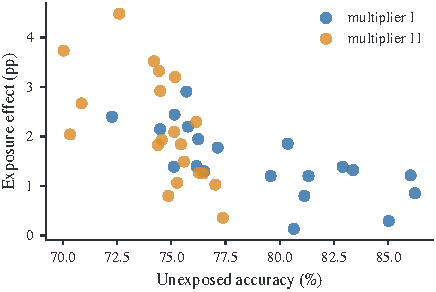
\includegraphics[width=0.52\textwidth]{figures/tmlrs_internal_heterogeneity.pdf}
\caption{Exploratory internal function effects against unexposed accuracy.
Color distinguishes the two affine multipliers.}
\label{tmlrs:fig:internal-heterogeneity}
\end{figure}

The normalized-gain contrast is substantial: exposure removes much less of
the remaining error in the internal setting than in CLUTRR.  This analysis
does not evaluate displacement on non-target functions.

\subsection{Historical Full-Protocol Contrast}

The following earlier comparison motivated the confirmatory intervention but
is not its substitute.  It jointly changes split unit, sampling prior, and
stratification, so its difference cannot be attributed only to aliases.

\begin{table}[H]
\caption{Historical full-protocol comparison, retained as context.  Accuracy
is percent, mean $\pm$ sample standard deviation over five matched seeds.
Legacy semantic is diagnostic, not a retrained protocol; the contrast changes
sampling prior and stratification as well as duplicate membership.}
\label{tab:supp-internal-models}
\centering
\small
\setlength{\tabcolsep}{2.2pt}
\resizebox{\textwidth}{!}{%
\begin{tabular}{lrrrrr}
\toprule
Architecture & Parameters & Legacy nominal & Legacy semantic & Strict function
& Nominal $-$ strict [95\% CI] \\
\midrule
Deep Sets \cite{zaheer2017deep} & 75,092 & $45.36{\pm}1.28$ & $41.27{\pm}1.25$ &
$38.86{\pm}0.86$ & $+6.50\ [5.02,7.99]$ \\
Relation Network \cite{sung2018relation} & 189,972 &
$72.13{\pm}1.37$ & $70.18{\pm}1.70$ &
$72.04{\pm}2.10$ & $+0.09\ [-3.06,3.25]$ \\
Set Transformer \cite{lee2019set} & 105,940 &
$64.36{\pm}1.45$ & $62.11{\pm}1.76$ &
$61.67{\pm}2.01$ & $+2.69\ [1.48,3.90]$ \\
Modern Hopfield-style \cite{ramsauer2021hopfield} & 72,340 &
$74.14{\pm}1.29$ & $72.32{\pm}1.23$ &
$72.93{\pm}1.63$ & $+1.21\ [-0.51,2.92]$ \\
Perceiver-style \cite{jaegle2021perceiver} & 141,780 &
$61.99{\pm}4.27$ & $59.93{\pm}5.05$ &
$57.93{\pm}1.94$ & $+4.06\ [-2.53,10.66]$ \\
Transformer \cite{vaswani2017attention} & 73,492 &
$67.54{\pm}2.00$ & $65.48{\pm}2.32$ &
$68.22{\pm}0.94$ & $-0.68\ [-2.40,1.05]$ \\
\midrule
Architecture macro & -- & 64.26 & 61.88 & 61.94 &
$+2.31\ [0.84,3.79]$ \\
\bottomrule
\end{tabular}
}
\end{table}

The architecture order is identical under legacy nominal and strict function
metrics: modern Hopfield-style, Relation Network, Transformer, Set
Transformer, Perceiver-style, then Deep Sets.  Spearman $\rho=1$ and maximum
rank movement is zero.

\subsection{Family Holdout}

\emph{Diagnostic context only; this contrast is not part of the audit
findings or of any behavioral claim in the main text.}

\begin{table}[H]
\caption{Known-family unseen-function and equal-family held-out performance.
Accuracy is percent.}
\label{tab:supp-family}
\centering
\scriptsize
\setlength{\tabcolsep}{3pt}
\begin{tabular}{lrrr}
\toprule
Model & Known & Held-out & Cross entropy \\
\midrule
Deep Sets & 38.86 & 8.14 & 6.366 \\
Relation Network & 72.04 & 11.23 & 6.942 \\
Set Transformer & 61.67 & 10.45 & 5.479 \\
Modern Hopfield & 72.93 & 11.33 & 5.990 \\
Perceiver & 57.93 & 10.85 & 6.609 \\
Transformer & 68.22 & 11.53 & 5.639 \\
Family Bayes & 98.60 & 99.17 & 0.018 \\
\bottomrule
\end{tabular}
\end{table}

The family-agnostic Bayesian mixture reaches 98.93\% posterior-expected
accuracy; changing to a uniform prior over unique maps changes this by only
0.04 points.  The family-transfer failure is therefore not explained by
insufficient information in eight noisy demonstrations.

\section{SLR-Bench Semantic Audit}

\subsection{Frozen Sources}

\begin{table}[H]
\caption{Frozen SLR audit inputs.  Individual Parquet SHA-256 values are stored
in the artifact manifest.}
\label{tab:slr-source}
\centering
\small
\begin{tabular}{p{0.78in}p{2.0in}}
\toprule
Object & Frozen value \\
\midrule
Repository & \texttt{ScalableLogicalReasoning} \\
Code revision & \texttt{3b46979ccdf9...} \\
Dataset & \texttt{AIML-TUDA/SLR-Bench}, configuration \texttt{v1-All} \\
Dataset revision & \texttt{cecc0aa26029...} \\
Rows & 18,053 train; 1,000 test \\
\bottomrule
\end{tabular}
\end{table}

\subsection{Token Identity}

After comments are removed, the Prolog lexer preserves atoms, variables,
punctuation, and operators while discarding whitespace.  Seventy large language
model (LLM)-guided test rules have a token sequence equal to a training rule.
The raw rule strings remain different, so verbatim overlap is zero.

\begin{verbatim}
% test
eastbound(T) :-
  has_car(T, C),
  (has_wall(C, full);
   car_color(C, yellow)).

% train: same Prolog tokens
eastbound(T) :-
  has_car(T, C),
  (has_wall(C, full);
   car_color(C, yellow)).
\end{verbatim}

\subsection{Flat Positive Rule Semantics}

A parsed flat positive rule has the form
\begin{equation}
\mathrm{eastbound}(t)\leftarrow
\bigwedge_j A_j(t,\mathbf z).
\end{equation}
For each existential car variable, we collect its unary attribute profile,
sort atoms within the profile, sort profiles, and alpha-rename variables.
Three successively stronger canonicalizations are used:
\begin{enumerate}
    \item alpha-renaming and conjunction-order normalization;
    \item idempotence of duplicate existential profiles;
    \item removal of a profile entailed by a stronger profile.
\end{enumerate}

Idempotence is sound because variables need not denote distinct objects:
\begin{equation}
\exists x\,P(x)\land\exists y\,P(y)
\equiv \exists x\,P(x).
\end{equation}
For profile sets $P\subseteq Q$,
\begin{equation}
\exists x\,Q(x)\land\exists y\,P(y)
\equiv \exists x\,Q(x),
\end{equation}
because an object satisfying $Q$ also witnesses $P$.

\begin{table}[H]
\caption{Progressive SLR overlap counts out of 1,000 test rows.  The flat-rule
parser covers 702 test and 13,568 training rows.}
\label{tab:slr-stages}
\centering
\small
\begin{tabular}{lr}
\toprule
Canonicalization & Overlapping test rows \\
\midrule
Alpha-renaming + atom order & 81 \\
+ existential idempotence & 369 \\
+ profile subsumption & 382 \\
Token identity (disjoint set) & 70 \\
\midrule
Sound union lower bound & \textbf{452} \\
\bottomrule
\end{tabular}
\end{table}

The union contains 382 random-generator rules and 70 LLM-guided rules, with
zero intersection.  It covers every test row at curriculum levels 1 and 3,
and remains nonzero through level 20.  Aggregate, negated, arithmetic, and
non-token-identical disjunctive rules are unresolved, so 45.2\% cannot be
interpreted as an exact total.

\subsection{Released Per-Item Output Caveat}

The repository \texttt{AIML-TUDA/Llama-3.1-8B-SLR} contains 1,000 per-item
outputs whose problem IDs and ground-truth rules align exactly with
\texttt{v1-All}.  A verifier mirroring the released extensional judge, run
with Trealla Prolog, gives the tier accuracies in
Table~\ref{tab:slr-output-mismatch}.

\begin{table}[H]
\caption{Tier accuracy mismatch.  Even treating all 30 Basic-tier runtime
errors as correct yields only 63.6\%, so runtime differences cannot explain
the final-paper gap.}
\label{tab:slr-output-mismatch}
\centering
\small
\begin{tabular}{lrrrr}
\toprule
Source & Basic & Easy & Medium & Hard \\
\midrule
Hosted per-item artifact & 51.6 & 55.2 & 20.4 & 5.2 \\
Association for Computational Linguistics (ACL) 2026 Table 2 & 96 & 54 & 18 & 5 \\
arXiv v2 Table 2 & 92 & 77 & 17 & 2 \\
\bottomrule
\end{tabular}
\end{table}

We therefore mark this artifact \texttt{exploratory\_only} and do not use it
to estimate the reported model's seen/unseen effect.

\subsection{Registered Association: Not Identified}

The confirmatory target was the final-paper
\texttt{Llama-3.1-8B-IT-SLR} result.  Before loading outcomes, the protocol
required a prediction source tied to a checkpoint and complete decoding
configuration, plus at least 80\% retention in both witnessed and no-witness
groups under exact curriculum-level common support.

No eligible prediction source was found.  The repository-hosted rows align
with all 1,000 test IDs and rules but do not reproduce the published main
table.  The common-support precheck also retains only 352/452 witnessed rows
(77.88\%), versus 498/548 no-witness rows (90.88\%).  The registered
propensity model, outcome model, and 10,000-replicate bootstrap were therefore
not run.  No adjusted association estimate, confidence interval, or direction
is reported.

\section{Boolean ICL Generator and Coverage Audit}

\subsection{Released Version}

The camera-ready paper \cite{bhattamishra2024understanding} points to
\texttt{satwik77/incontext-bool}.  We freeze revision
\texttt{a25a2cb0c62...}; its
\texttt{bool\_tasks.py} SHA-256 is
\texttt{5bda5cdb00bc...}.  Full hashes are frozen in the source manifest.
The core task abstract syntax trees (ASTs) match the camera-ready supplementary
archive.  No checkpoint or per-function evaluation output is released.

\begin{table}[H]
\caption{Paper/released-code differences.  The behavioral intervention uses
only the frozen released definitions and is not presented as a reproduction
of unreleased main-table configurations.}
\label{tab:boolean-mismatch}
\centering
\small
\setlength{\tabcolsep}{3.2pt}
\begin{tabular}{p{1.0in}p{2.3in}p{2.3in}}
\toprule
Task & Camera-ready description & Released code \\
\midrule
Sparse Disjunction &
$n=50$, at most three signed literals &
Exactly four literals, positive only \\
Sparse Parity &
Main table includes $(10,2)$ and $(20,3)$ &
Sampler hard-codes $k=2$ and ignores a $k$ argument \\
0--1 Threshold &
Uniform weights and seven integer thresholds &
Weights use $(0.7,0.15,0.15)$ and six half-integer thresholds \\
Registry &
0--1 Threshold / Integer Halfspace task labels &
Names are \texttt{sparse\_thres} / \texttt{int\_halfspace}; bundled
alternative names are unregistered \\
\bottomrule
\end{tabular}
\end{table}

\subsection{Exact Semantic IDs}

For Conjunction-28, the semantic ID is the vector
$w\in\{0,+1,-1\}^{28}$; exhaustive small-dimension truth tables verify
injectivity, and differing signed literal sets can be separated by an input.
For Majority-28, the ID is the active-variable bit mask.  For released Sparse
Disjunction-50, the ID is the four-element positive-literal subset.  Any two
different subsets are separated by assigning a differing literal true and
the other subset's literals false.  Thus the IDs are exact for these released
families without enumerating $2^{28}$ or $2^{50}$ inputs.

At the frozen budget $N=20{,}000\times32=640{,}000$, the analytic exposure
probabilities from Equation~\ref{eq:supp-coverage} are 0.914\%, 9.457\%, and
93.790\%.  The actual frozen streams give the values in
Table~\ref{tab:boolean-exposure}.

\begin{table}[H]
\caption{Percentage of the 1,280 frozen evaluation draws whose semantic ID
appears in each Original training stream.  Every Strict value is zero.}
\label{tab:boolean-exposure}
\centering
\small
\begin{tabular}{lrrrr}
\toprule
Task & Seed 0 & Seed 1 & Seed 2 & Mean \\
\midrule
Conjunction & 0.94 & 0.70 & 0.78 & 0.81 \\
Majority & 8.83 & 8.28 & 9.53 & 8.88 \\
Sparse Disjunction & 93.05 & 92.81 & 94.45 & 93.44 \\
\bottomrule
\end{tabular}
\end{table}

\section{Boolean Behavioral Intervention}

\subsection{Preregistration and Pairing}

Before training, we froze:
\begin{itemize}
    \item 1,280 evaluation function draws and prompt seeds per task;
    \item three 640,000-function Original streams;
    \item Strict streams that replace only slots colliding with any evaluation
    semantic ID;
    \item model seeds, input random-number streams, optimizer, budget, primary
    endpoint, bootstrap procedures, and success criteria.
\end{itemize}

The model is the released Transformer implementation configured with six
layers, hidden size 256, eight heads, no dropout, and float32 precision.
Training uses Adam with learning rate $10^{-4}$, batch size 32, 40 points per
episode, and 20,000 fixed steps.  No validation selection is used.  The final
checkpoint is evaluated on the same prompts under both protocols.

The primary endpoint is mean sign accuracy over zero-indexed positions
20--39.  The effect is
\begin{equation}
\Delta_{\rm pp}=100(A_{\rm Original}-A_{\rm Strict}).
\end{equation}
The core criterion requires one task with mean $\Delta_{\rm pp}\geq2$ and all three seed
deltas positive.  The strong-pattern criterion additionally requires Sparse Disjunction
$\geq5$ points, absolute Conjunction effect $\leq2$ points, and nondecreasing
effects across the exposure gradient.  Confidence intervals are reported but
do not determine the decision.

\subsection{Complete Primary Results}

\begin{table}[H]
\caption{Per-seed primary results.  Each interval uses 10,000 paired
semantic-ID cluster bootstrap replicates.}
\label{tab:boolean-per-seed}
\centering
\scriptsize
\setlength{\tabcolsep}{3.4pt}
\begin{tabular}{llrrrrr}
\toprule
Task & Seed & Exposure (\%) & Original (\%) & Strict (\%) &
$\Delta$ (pp) & Cluster-bootstrap 95\% CI \\
\midrule
\multirow{3}{*}{Conjunction}
& 0 & 0.94 & 92.871 & 92.875 & -0.004 & $[-0.094,0.090]$ \\
& 1 & 0.70 & 93.059 & 93.117 & -0.059 & $[-0.203,0.086]$ \\
& 2 & 0.78 & 92.902 & 92.879 & +0.023 & $[-0.004,0.051]$ \\
\midrule
\multirow{3}{*}{Majority}
& 0 & 8.83 & 78.379 & 78.520 & -0.141 & $[-0.324,0.039]$ \\
& 1 & 8.28 & 78.852 & 78.953 & -0.102 & $[-0.281,0.078]$ \\
& 2 & 9.53 & 79.223 & 79.172 & +0.051 & $[-0.129,0.230]$ \\
\midrule
\multirow{3}{*}{Sparse Disjunction}
& 0 & 93.05 & 81.387 & 81.418 & -0.031 & $[-0.180,0.125]$ \\
& 1 & 92.81 & 83.613 & 83.367 & +0.246 & $[-0.023,0.516]$ \\
& 2 & 94.45 & 81.949 & 81.887 & +0.063 & $[-0.078,0.203]$ \\
\bottomrule
\end{tabular}
\end{table}

\begin{table}[H]
\caption{Three-seed primary summaries in percentage points.  Hierarchical
intervals use 20,000 replicates, resampling model seeds and semantic-ID
clusters.}
\label{tab:boolean-summary}
\centering
\scriptsize
\setlength{\tabcolsep}{2.6pt}
\begin{tabular}{lrrr}
\toprule
Task & Mean & Hier. CI & $t_2$ CI \\
\midrule
Conjunction & -0.013 & $[-0.092,0.044]$ & $[-0.117,0.091]$ \\
Majority & -0.064 & $[-0.199,0.078]$ & $[-0.315,0.187]$ \\
Sparse Disj. & +0.092 & $[-0.060,0.282]$ & $[-0.258,0.443]$ \\
\bottomrule
\end{tabular}
\end{table}

No task reaches 2 points or has three positive deltas.  Neither the core
nor the strong-pattern criterion is met.  The registered Transformer seed
expansion and long short-term memory (LSTM) ranking experiment are not
triggered.

\subsection{Secondary Endpoints}

\begin{table}[H]
\caption{Three-seed secondary means, Original minus Strict.  Negative binary
cross-entropy (BCE) favors Original because lower is better.  Secondary
endpoints do not replace the registered primary criterion.}
\label{tab:boolean-secondary}
\centering
\scriptsize
\setlength{\tabcolsep}{3pt}
\begin{tabular}{lrrr}
\toprule
Task & Final & Pos. 1--39 & Tail BCE \\
\midrule
Conjunction & +0.052 pp & +0.011 pp & +0.0007 \\
Majority & -0.130 pp & -0.072 pp & -0.0001 \\
Sparse Disj. & +0.156 pp & +0.073 pp & -0.0019 \\
\bottomrule
\end{tabular}
\end{table}

Within Original runs, seen-versus-unseen accuracy is descriptive only:
exposure is not randomized and the groups differ substantially in size.  We do not
use this stratification as a substitute for the paired intervention.

\subsection{Integrity Validation}

All 18 runs completed 20,000 steps.  A separate validation code path checks:
\begin{itemize}
    \item frozen source, adapter, manifest, and stream hashes;
    \item finite model and optimizer tensors;
    \item 1,280 finite per-episode logits per run;
    \item zero Strict semantic exposure;
    \item identical paired evaluation semantic IDs, labels, and Original
    exposure flags;
    \item complete finite training logs and artifact SHA-256 values.
\end{itemize}
All checks pass.  The compact analysis contains 11,520 paired episode rows.
The 1.9\,GB checkpoints are not required to reproduce the reported statistics
and are excluded from the public artifact.

\section{Registration Timeline}
\label{app:registration-timeline}

Rows are listed in evidential order and are not pooled as one sequential
experiment.  Each row states what was frozen before the corresponding
outcomes were observed and which earlier decision later work does not revise.

\begin{table}[H]
\caption{Registration timeline.  Each study was frozen before its outcomes
were observed; later studies do not revise earlier decisions.}
\label{tab:stage-timeline}
\centering
\scriptsize
\setlength{\tabcolsep}{2pt}
\begin{tabular}{L{0.85in}L{1.45in}L{1.8in}L{1.45in}}
\toprule
Study & Frozen before outcomes & Role and outcome & Not revised by later work \\
\midrule
Internal intervention &
Paired streams, endpoints, and success criteria before training &
Confirmatory exact-alias intervention; preregistered macro criterion met &
Later public studies do not alter it \\
SLR-Bench &
Source artifacts and identification rules before outcome modeling &
Structural 45.2\% lower bound; association analysis stopped at its
preregistered identification check &
No later outcome substitutes for the stopped analysis \\
Original breadth scope (Tensor Logic, Occam) &
Candidates before semantic extraction &
Prospective structural audits; breadth criterion not met &
CLUTRR uses a new scope and does not reopen it \\
Toolkit and theory validation &
Schema tests and certificate assumptions before validation runs &
Validate reporting machinery &
Do not change the breadth decision \\
CLUTRR V3 &
Targets, training, endpoint, bootstrap, and precision criterion &
Preregistered pilot; positive but imprecise &
The positive direction is not relabeled as success \\
V3 diagnosis &
Exploratory status declared after V3 was closed &
Post-unblinding variance analysis &
Designs V4 but cannot change V3 \\
CLUTRR V4 &
V3-disjoint targets and directional criterion before materialization and
training &
Prospective confirmation; directional criterion met &
Not pooled with V3 \\
\bottomrule
\end{tabular}
\end{table}

\section{Original Prospective Public-Benchmark Scope}

Candidate discovery queried Semantic Scholar and arXiv using four frozen
strings, deduplicated by DOI, arXiv ID, then normalized title, and screened in
ascending title order.  The manifest was frozen before candidate code or data
were semantically inspected.  Both selected candidates are reported; neither
was removed after its result was known.

\subsection{Tensor Logic FB15k-237}

We pin the Tensor Logic code at revision
\texttt{9b497c279928...} and FB15k-237 at
\texttt{2e440e0f9c68...}.  Experiment 3B first selects 2,000 unique endpoint
pairs with two-hop paths, splits them equally into validation and test, and
then removes all corresponding direct triples from training.  The code does
not revalidate whether removing one direct triple destroys an edge used by a
different selected path.

\begin{table}[H]
\caption{Tensor Logic path audit, out of 1,000 rows per split.  Endpoint and
relation-schema witnesses answer different semantic questions.}
\label{tab:tensor-audit}
\centering
\small
\begin{tabular}{lrr}
\toprule
Audit quantity & Validation & Test \\
\midrule
Direct edge absent after scrub & 1,000 & 1,000 \\
Designated two-hop path retained & 336 & 379 \\
Any exact endpoint witness retained & 441 & 484 \\
Relation schema seen in scrubbed train & 994 & 999 \\
No retained endpoint witness & 559 & 516 \\
\bottomrule
\end{tabular}
\end{table}

Thus direct-edge withholding succeeds, but the claim that every evaluation
query retains its generating two-hop path fails.  Under the certified
interval below, the test split has endpoint exposure in
$[484,1000]/1000$ and relation-schema exposure in
$[999,1000]/1000$.  No public checkpoint, per-item ranks/predictions, or
training logs were found, so this is a protocol-level audit without credible
behavioral evidence.

\subsection{In-Context Occam's Razor}

We pin the public repository at revision
\texttt{3b8fe0d69dd9...}.  Its Markov training generator assigns task seed
\texttt{step+i}; the evaluator fixes ten seeds
\(s_j=12574j+5\) for every tested order and draws 100 sequences per task.
The paper's 800,000-sequence horizontal axis and batch size 32 imply 25,000
nominal steps, hence training seed support \(0,\ldots,25030\).

Seeds 5 and 12,579 occur six and 32 times, respectively.  Because the
category assignment chooses between the two trained orders but uses unseeded
NumPy state, the exact exposed order identities are unavailable.  For each
supported seed, however, at least one and at most both evaluated orders occur
in training.  An exhaustive census recomputes 75,093 transition signatures
(25,031 seeds for orders 1, 2, and 3) and finds no cross-seed collision.
Consequently both main experiments have exact latent-task exposure
\([2,4]/20=[10\%,20\%]\), corresponding to 200--400 of 2,000 evaluation
sequences.

The same seed rule creates 800,000 training episodes from only 25,031 seed
IDs.  Even if every seed realizes both orders whenever possible, there are at
most 50,060 distinct \texttt{(order, transition tensor)} tasks, so at least
749,940/800,000 (93.7425\%) episodes reuse a latent task.  The repository has
no linear-regression generator, training, evaluation, or curriculum code,
although regression is part of the frozen candidate scope.  That scope is
therefore unresolved and the candidate is not a complete audit under the
original breadth scope.

\subsection{Frozen Breadth Decision}

Tensor Logic counts as one complete public semantic audit; the Occam
candidate does not because its required regression half is unavailable.
Neither candidate has a controlled intervention or reproducible per-item
behavioral source.  The frozen breadth scope therefore has one of two required
complete audits and zero of one required behavioral benchmarks, so the
breadth criterion is not met.  This historical decision does not discard
either case and is not
changed by the later, independently preregistered CLUTRR expansion.

\section{CLUTRR External Behavioral Validation}
\label{app:clutrr}

\subsection{Frozen Scope and Semantic Identity}

Both studies use CLUTRR Task~1 at relation length three, without distractor
facts.  A row contains three kinship-relation sentences and one queried
relation from 23 output classes.  Entity names are canonicalized by order of
appearance.  The semantic ID is
\[
(\text{target relation},
 \text{edge relation}_1,
 \text{edge relation}_2,
 \text{edge relation}_3),
\]
where the edges follow the ordered proof chain.  Sentence order and entity
surface names are excluded from this ID.

For each source story, all six sentence permutations receive one shared
\texttt{source\_group\_id}.  Eligible targets have at least 45 complete
groups.  The evaluation rows use the first 34 groups after deterministic
sorting: six permutations from groups 0--32 and two from group~33, for 200
rows per target.  Exposure uses the next 11 groups: six permutations from
groups 34--43 and four from group~44, for 64 rows per target.  Thus no source
group contributes to both exposure and evaluation.

Targets are paired only when they have the same output label.  For each seed,
a frozen SHA-256 bit assigns one member of every pair to each arm.  The two
arms share 22,720 common-base rows with no target semantic ID and append
1,280 exposure rows, giving 24,000 rows per run.  Label histograms, total
budget, tensor shape, initialization, epoch orders, and evaluation rows are
paired.

\subsection{Model, Training, and Primary Analysis}

The model is a byte-level Transformer with four layers, model dimension 128,
four attention heads, feed-forward dimension 512, dropout 0.1, pooling over a
classification token, and 23 output classes.  Training uses deterministic CPU
float32 execution, AdamW, batch size 128, learning rate
$3\times10^{-4}$, and 30 fixed epochs.  Each epoch contains 188 updates, so
the final checkpoint follows 5,640 updates.  There is no validation selection
or early stopping.

For seed $s$, let $\mathbf Z_s^A$ be the complete target-exposure assignment
in Arm~A and let $\mathbf Z_s^B=\mathbf 1-\mathbf Z_s^A$.  For target $f$,
$\mathbf Z_{s,f}^{(1)}$ is whichever arm assignment exposes $f$, and
$\mathbf Z_{s,f}^{(0)}$ is the complementary assignment.  Let
$A_{s,f}(\mathbf z)$ be row-weighted accuracy under complete curriculum
assignment $\mathbf z$.  The primary estimand is
\begin{equation}
\tau_{\rm pp}
=
\frac{100}{SF}
\sum_{s=1}^{S}\sum_{f=1}^{F}
\left[
A_{s,f}(\mathbf Z_{s,f}^{(1)})
-A_{s,f}(\mathbf Z_{s,f}^{(0)})
\right].
\end{equation}
Targets and seeds have equal weight; each target's 200 evaluation rows have
equal weight.  This target-indexed estimand compares two complete,
complementary curricula; it does not identify a one-target direct effect while
holding the other target assignments fixed.

The 20,000-replicate percentile bootstrap resamples model seeds, complete
same-label semantic-pattern pairs, and source groups within each selected
pair member.  Exposed and unexposed predictions use the same group draws, and
all rows from a sampled group occurrence remain together.  Percentiles use
NumPy's linear quantile method.  A separate analysis code path reconstructs
arm alignment from materialized assignments rather than trusting stored arm
labels.

The estimand itself is finite-population: it averages the eight frozen seeds
and 80 frozen targets.  For interval construction, the bootstrap treats the
observed seed labels, 40 complete pair labels, and source-group labels within
each target as exchangeable under their empirical distributions.  The
justification is procedural symmetry after freezing: each seed uses the same
architecture and training protocol, each selected pair receives the same
complementary intervention, and source-group IDs only identify permutations
of one source story.  Seed and pair resampling preserve their complete
clusters; group draws and duplicate seed occurrences are shared across arms.
The deterministic target-prefix and source-group allocation prevent a
design-based interpretation for all eligible CLUTRR patterns or stories.

The post-hoc sensitivity analysis uses the 640 seed-pattern effects
\(d_i\).  With residual
\(u_i=d_i-\bar d\), each cluster dimension \(c\) has CR1 variance
\[
\widehat V_c=
\frac{G_c}{G_c-1}\frac{1}{N^2}
\sum_{g=1}^{G_c}\left(\sum_{i\in g}u_i\right)^2.
\]
Clustering by model seed and complete pattern pair gives
\(\widehat V_{\rm two-way}
=\widehat V_{\rm seed}+\widehat V_{\rm pair}
-\widehat V_{\rm seed\times pair}\).
The resulting standard error is 2.6187 points.  A conservative two-sided
\(t_7\) interval is \([17.1469,29.5313]\) points, still above zero.  This
post-hoc sensitivity is not a new decision rule or a replacement for the registered
hierarchical bootstrap.

\subsection{V3 Pilot and Frozen Precision Decision}

V3 contains 20 pattern pairs, 40 targets, eight seeds, and two arms, for 16
runs and 128,000 saved evaluation predictions.  Before outcomes, the protocol
required any positive, negative, or equivalence conclusion to have a 95\%
interval no wider than two percentage points.

\begin{table}[H]
\caption{V3 primary result and registered decision.}
\label{tab:app-clutrr-v3}
\centering
\small
\begin{tabular}{lr}
\toprule
Quantity & Value \\
\midrule
Point estimate & $+15.3375$ pp \\
95\% percentile interval & $[+9.8769,+21.3693]$ pp \\
Interval width & $11.4924$ pp \\
Frozen maximum width & $2.0000$ pp \\
Registered outcome & positive but imprecise (precision criterion not met) \\
\bottomrule
\end{tabular}
\end{table}

The V3 estimand averages eight frozen seeds and 40 frozen targets.  Conditional
on that setting, its bootstrap treats those seeds, 20 complete pairs, and
within-target source groups as exchangeable empirical draws while preserving
clusters and paired arms.  Deterministic selection precludes design-based
generalization to all eligible CLUTRR patterns or stories.

The interval is directionally positive but fails the registered precision
criterion.  That decision is retained without reinterpretation.

After V3 was closed, a labeled exploratory analysis used bootstrap-Shapley
variance attribution and a seed-by-pair random-effects decomposition.
Pattern-pair resampling accounts for 94.40\% of bootstrap variance, compared
with 4.90\% for model seeds and 0.70\% for source groups.  The random-effects
estimates are $162.6402$ pp$^2$ for pair heterogeneity, $0.3490$ pp$^2$ for
seeds, and $48.6744$ pp$^2$ for the seed-by-pair interaction.

\subsection{Exploratory Effect Heterogeneity}
\label{tmlrs:app:clutrr-heterogeneity}

This exploratory (not preregistered) analysis resolves the V4 contrast into
its \TTwoPatterns{} semantic patterns.  The pattern effects have mean
\TTwoMean{} pp,
median \TTwoMedian{} pp, sample standard deviation \TTwoSD{} pp, and range
\TTwoMin{}--\TTwoMax{} pp; \TTwoPositive{}/\TTwoPatterns{} are positive.
Effect size is
strongly associated with unexposed accuracy
(Spearman $\rho=\TTwoSpearman{}$).  A linear regression on that baseline
alone has $R^2=\TTwoBaseRSquared{}$; adding target-relation indicators raises
it to $R^2=\TTwoRelationRSquared{}$.  The median normalized gain is
\TTwoNGMedian{}, so the raw spread is not only a scale artifact, although
available headroom explains much of it.

Mean effects are \TTwoInAbsentMean~pp when the target relation is absent
from the three edges (\TTwoInAbsentN{} patterns) and \TTwoInPresentMean~pp
when it is present (\TTwoInPresentN), and \TTwoDistinctOneMean,
\TTwoDistinctTwoMean, and \TTwoDistinctThreeMean~pp for one, two, and three
distinct edge types (\TTwoDistinctOneN, \TTwoDistinctTwoN, and
\TTwoDistinctThreeN{} patterns).  Neither covariate predicts the effect at
conventional levels (two-sided Spearman $p=\TTwoInP{}$ and
$p=\TTwoDistinctP{}$, respectively).
Target relation as a categorical grouping explains \TTwoEta{} of the effect
variance, but
leave-one-relation mean effects remain within
\TTwoLeaveMin{}--\TTwoLeaveMax{} pp.  Figure
\ref{tmlrs:fig:clutrr-heterogeneity} shows the full distribution.  Exposure
gains are largest where the unexposed model is far from ceiling, and
normalized gain is high for most patterns; the heterogeneity is thus mostly
a headroom effect rather than evidence for a particular compositional
mechanism.

A calibrated prospective projection finds that the original two-point width
would require about 634 independent pairs even with infinitely many seeds.
Only 139 eligible V3-disjoint pairs remain, and using all of them with
infinitely many seeds projects to a 4.2690-point width.  The strict-precision
replication route was therefore closed rather than consuming more seeds under
an infeasible criterion.

\subsection{Prospective V4 Design}

V4 treats V3 as a declared pilot and changes the scientific question from a
two-point precision target to directional confirmation.  The prospective
design effect is
\[
\min(0.5\times15.3375,\;9.8769)=7.66875\ \text{pp}.
\]
A 100,000-draw 64-bit permuted congruential generator (PCG64) Monte Carlo
simulation evaluates one to four 20-pair blocks.  The frozen selection rule
chooses the smallest block count for which estimated power and the 95\% Wilson
lower confidence bound are both at least 0.90.

For candidate pair count \(Q\in\{20,40,60,80\}\), set the frozen design
effect to \(\delta=7.66875\) points and draw
\[
\begin{aligned}
\widehat\tau_Q&=\delta+\mathrm{SE}_Q Z,\qquad Z\sim N(0,1),\\
\mathrm{SE}_Q
&=c\sqrt{
\frac{\sigma_s^2}{8}
+\frac{\sigma_p^2}{Q}
+\frac{\sigma_{sp}^2}{8Q}
}.
\end{aligned}
\]
The V3 random-effects inputs are
\(\sigma_s^2=0.3490014\),
\(\sigma_p^2=162.6401609\), and
\(\sigma_{sp}^2=48.6744361\) pp\(^2\), with frozen calibration
\(c=1.0067880\).  The seed effect is shared across pairs, the pair effect
across seeds, and the interaction is seed-by-pair.  Source groups are nested
within targets and shared across arms; their contribution is not a fourth
explicit random effect, but enters \(c\) through calibration to the full V3
hierarchical percentile width, which resampled source groups.  A simulated
experiment succeeds exactly when
\(\widehat\tau_Q\geq1\) and
\(\widehat\tau_Q-1.959964\,\mathrm{SE}_Q>0\).
Power is the fraction of 100,000 successful draws; the block-size rule additionally
requires its binomial 95\% Wilson lower endpoint to be at least 0.90.

\begin{table}[H]
\caption{V4 power analysis for the first two candidate sizes.}
\label{tab:app-clutrr-power}
\centering
\small
\begin{tabular}{rrrrr}
\toprule
Blocks & Pairs & Runs & Power & Wilson lower \\
\midrule
1 & 20 & 16 & 0.74397 & 0.74126 \\
2 & 40 & 32 & 0.95828 & 0.95702 \\
\bottomrule
\end{tabular}
\end{table}

The minimum-passing design therefore has two blocks, 40 pairs, 80 patterns,
and 32 runs.  All target semantic IDs are disjoint from V3.  The primary success criterion,
frozen before materialization and training, requires
\(\tau_{\rm pp}\geq1\) and a two-sided 95\% interval lower endpoint above
zero.

\subsection{V4 Execution Integrity and Result}

Materialization validates 80 targets, 16,000 evaluation rows across two
blocks, 5,120 exposure rows, the shared 22,720-row common base, and all 32
training manifests.  The frozen execution assets include a
$43{,}840\times185$ tensor cache, 32 arrays of 24,000 training indices,
two 8,000-row evaluation caches, eight initialization records, and 240
epoch-order records.

All 32 runs reach epoch 30.  The post-execution validator checks finite model
and optimizer state, 960 run-by-epoch order records, 256,000 predictions,
four-way RNG pairing across both blocks and arms within each seed, prediction
ordering, separate-code-path metric reconstruction, and artifact hashes.

\begin{table}[H]
\caption{V4 primary and descriptive results.  Sign counts do not define
additional hypothesis tests.}
\label{tab:app-clutrr-v4}
\centering
\small
\begin{tabular}{lr}
\toprule
Quantity & Value \\
\midrule
Point estimate & $+23.3391$ pp \\
95\% percentile interval & $[+17.7498,+29.2257]$ pp \\
Registered outcome & directional criterion met \\
Block effects & $+25.0109,\ +21.6672$ pp \\
Positive seeds & 8/8 \\
Positive pairs & 40/40 \\
Positive target patterns & 76/80 \\
Cross entropy, exposed minus unexposed & $-1.4938$ \\
Brier score, exposed minus unexposed & $-0.4224$ \\
ECE-15, exposed minus unexposed & $-0.2018$ \\
\bottomrule
\end{tabular}
\end{table}

The V4 point estimate exceeds one point and its interval lies above zero, so
the registered directional positive rule passes.  V3 and V4 are not pooled:
they use disjoint targets, answer different registered decision questions,
and retain separate bootstrap draws and classifications.

\subsection{Paper Artifact}

The compact CLUTRR bundle contains 51 checksum-managed files:
design and effect preregistrations, freeze validations, execution-integrity
reports, run-artifact hashes, exact bootstrap draws, pair/pattern/seed tables,
code snapshots, claim boundaries, source-file provenance, and a standalone
verifier.  It excludes local paths and large checkpoints.  Its
\texttt{SHA256SUMS} file has SHA-256
\texttt{210dddc02840a7bab7fe1215378d36ac\allowbreak86cc574a06aeca238482eab86ba3ef36}.


\section{Exploratory Semantic Versus Surface Exposure}
\label{tmlrs:app:semantic-surface}

This exploratory (not preregistered) intervention uses the \TSixPatterns{}
block-0 CLUTRR patterns and their shared 8,000-row evaluation set.  Every
arm appends 48 relation-matched rows per pattern to the same 22,720-row
common base, giving 24,640 training rows with identical label counts.
Arm C0 uses semantically unrelated filler rows.  Arm C1 uses eight complete
source-story groups with the target semantic identity.  Arm C2 uses distinct
semantic identities with the same target relation and at least two matching
edge types as a multiset.  All patterns met this strict two-edge criterion;
no one-edge fallback or main-analysis exclusion was needed.

The four seeds share initialization and epoch order across arms.  The model,
optimizer, and 30-epoch budget match the V4 configuration; execution uses
deterministic float32 Metal Performance Shaders.  The protocol was frozen
before training at hash prefix \texttt{\TSixProtocolHash}; its one-epoch
timing run took \TSixTimingSeconds{} seconds.  Pattern-cluster intervals use
2,000 resamples with seed zero, and seed intervals are paired
$t_3$ intervals.

The mean arm accuracies are \TSixCZeroAcc{}\% for C0,
\TSixCOneAcc{}\% for C1, and \TSixCTwoAcc{}\% for C2.

\begin{table}[H]
\caption{Exploratory semantic-versus-surface contrasts in percentage points.}
\label{tmlrs:tab:semantic-surface}
\centering
\small
\begin{tabular}{lrrr}
\toprule
Contrast & Effect & Pattern 95\% CI & Seed 95\% $t$ CI \\
\midrule
C1 $-$ C0 & \TSixSemGain{} &
$[\TSixSemLo{},\TSixSemHi{}]$ &
$[\TSixSemSeedLo{},\TSixSemSeedHi{}]$ \\
C2 $-$ C0 & \TSixDecoyGain{} &
$[\TSixDecoyLo{},\TSixDecoyHi{}]$ &
$[\TSixDecoySeedLo{},\TSixDecoySeedHi{}]$ \\
C1 $-$ C2 & \TSixSemDecoyGain{} &
$[\TSixSemDecoyLo{},\TSixSemDecoyHi{}]$ &
$[\TSixSemDecoySeedLo{},\TSixSemDecoySeedHi{}]$ \\
\bottomrule
\end{tabular}
\end{table}

\begin{figure}[H]
\centering
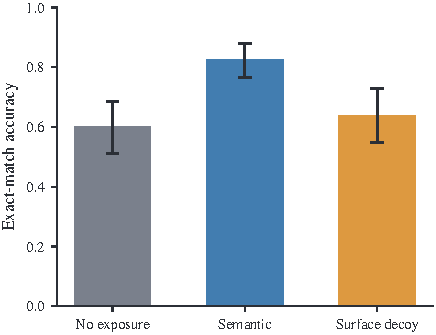
\includegraphics[width=0.52\textwidth]{figures/tmlrs_semantic_vs_surface.pdf}
\caption{Exploratory accuracy under no target exposure, same-semantic
exposure, and surface-similar decoys.  Bars show mean accuracy;
error bars are 95\% pattern-cluster intervals.}
\label{tmlrs:fig:semantic-surface}
\end{figure}

The pattern interval for C2--C0 is positive, although its four-seed
$t$ interval includes zero, so the decoys are not treated as having exactly
no effect.  More importantly, C1 exceeds C2 by \TSixSemDecoyGain{} pp with
pattern interval [\TSixSemDecoyLo{}, \TSixSemDecoyHi{}].  Under the
decision rule frozen in the protocol before training (not publicly
preregistered), this supports the interpretation that semantic identity,
not surface similarity alone, is the primary source of the gain in this
intervention.  The result remains bounded to these patterns, decoy criteria,
architecture, and training budget.

\section{Certified Exposure Intervals}
\label{app:certified}

\subsection{Assumptions and Proposition}

Fix one semantic namespace and evaluation identities
\(E=\{e_1,\ldots,e_N\}\).  Let \(z_i=1\) if evaluation identity \(e_i\)
occurs semantically in training, and \(z_i=0\) otherwise.
Assume: (A1) the finite denominator is frozen before inspection; (A2) every
identity has a deterministic canonical semantic ID; (A3) each executable
certificate supplies a sound constraint
\(\ell_j\leq\sum_{i\in G_j}z_i\leq u_j\); (A4) certificate groups are
pairwise disjoint; and (A5) uncovered identities receive no constraint beyond
binary membership.
Appendix~\ref{tmlrs:app:overlap} relaxes A4 computationally: mixed-integer
linear programming gives exact bounds for tractable overlapping systems,
while a linear-programming relaxation gives a dual-certified outer interval.

\paragraph{Proposition~\ref{prop:certified} (restated).}
Let \(R=E\setminus\cup_jG_j\).  Then
\begin{equation}
\sum_j\ell_j
\leq
C(E):=\sum_{i=1}^{N}z_i
\leq
|R|+\sum_j u_j.
\label{eq:supp-certified}
\end{equation}
Both endpoints are attained by some exposure assignment consistent with the
certificate system, so no tighter interval follows from the certificates
alone.

\paragraph{Proof.}
Disjointness partitions the total:
\[
C(E)=
\sum_j\sum_{i\in G_j}z_i+\sum_{i\in R}z_i.
\]
Applying each lower certificate and
\(\sum_{i\in R}z_i\geq0\) gives the lower bound.  Applying each upper
certificate and binary membership
\(\sum_{i\in R}z_i\leq|R|\) gives the upper bound.  To attain the endpoints,
choose
exactly \(\ell_j\) exposed identities in each \(G_j\) and none in \(R\);
this feasible assignment attains the lower endpoint.  Choosing exactly
\(u_j\) in each group and every identity in \(R\) attains the upper endpoint.
No tighter universal interval follows from these certificates alone.
\(\square\)

\subsection{Grouped-Seed Corollary}

For a fixed seed \(s\), suppose
\(G_s=\{\phi(1,s),\ldots,\phi(K,s)\}\) contains all evaluated categories,
every training episode using \(s\) selects exactly one member of \(G_s\), and
\(s\) appears \(m_s\) times.  If a complete signature census excludes
cross-seed aliases, then \(m_s=0\) gives group constraint \([0,0]\), while
\(m_s>0\) gives
\begin{equation}
1\leq\sum_{i\in G_s}z_i\leq\min(K,m_s).
\end{equation}
The lower bound follows because at least one category was selected; the upper
bound follows because at most \(K\) categories and at most \(m_s\) distinct
episode assignments can occur.  Persisting category assignments would
collapse this interval to the exact number of observed categories.

\subsection{Novelty-Conditioned Score Interval}
\label{tmlrs:app:novelty-proof}

Let $\mathcal R$ contain $M$ unresolved items with observed scores
$y_i\in[0,1]$, and let the unknown truly novel subset be
$\mathcal N\subseteq\mathcal R$.  Suppose external information only implies
$|\mathcal R\setminus\mathcal N|\leq U<M$, and write the ordered scores as
$y_{(1)}\leq\cdots\leq y_{(M)}$.

\paragraph{Proof.}
Fix $n=|\mathcal N|$.  Among all subsets of size $n$, replacing any selected
score by a smaller unselected score cannot increase the mean.  Repeating this
exchange shows that the minimum is the mean of the first $n$ order
statistics.  The symmetric exchange gives the maximum as the mean of the
last $n$ order statistics.

The mean of the first $n$ scores is nondecreasing in $n$: the next score
$y_{(n+1)}$ is no smaller than any of the first $n$ and hence no smaller than
their mean.  Because the exposure constraint permits
$n\in\{M-U,\ldots,M\}$, the global minimum is therefore attained at
$n=M-U$.  The corresponding upper-tail mean is nonincreasing in $n$, so the
global maximum is also attained at $n=M-U$.  Thus
\[
L(U)=\frac{1}{M-U}\sum_{k=1}^{M-U}y_{(k)},\qquad
H(U)=\frac{1}{M-U}\sum_{k=U+1}^{M}y_{(k)}.
\]
Taking $\mathcal N$ to be the first or last $M-U$ ordered items attains the
respective endpoint while excluding exactly $U$ items.  Increasing $U$
removes an upper-tail item from the lower construction or a lower-tail item
from the upper construction, so $L(U)$ is nonincreasing and $H(U)$ is
nondecreasing.  At $U=0$, both equal the observed mean. \(\square\)

For binary scores with $k$ correct items and $n=M-U$, this reduces to
\[
L(U)=\frac{\max(0,k-U)}{n},\qquad
H(U)=\frac{\min(k,n)}{n}.
\]
The exposure upper endpoint from Proposition~\ref{prop:certified} can be
used as $U$ when it applies to the unresolved set and is smaller than $M$.
If the available upper bound permits all $M$ items to be exposed, a novel
mean need not exist; conditional on a nonempty novel set, the interval is
$[\min_i y_i,\max_i y_i]$.  The construction is a finite trimming
argument related to \citet{lee2009training} and the contaminated-data bounds
of \citet{horowitz1995identification}.

\paragraph{Parameterized SLR sensitivity.}
The structural audit leaves $M=\TTenM{}$ items unresolved.  We use only
this denominator, not model predictions or partial scores.  Let $p=k/M$
be an unspecified correct fraction.  For integer $U<M$,
\[
L(p,U)=\frac{\max(0,pM-U)}{M-U},\qquad
H(p,U)=\frac{\min(pM,M-U)}{M-U}.
\]
For finite binary scores, $pM$ must be an integer; this condition preserves
endpoint attainment.  The bounds express a hypothetical sensitivity
calculation, not an observed accuracy or an estimated exposure rate.

Writing $\rho=U/M$, the greatest possible width over admissible $p$ is
\[
W_{\max}(U)=\max_{k\in\{0,\ldots,M\}}
\{H(k/M,U)-L(k/M,U)\}
=\min\left(1,\frac{U}{M-U}\right)
=\min\left(1,\frac{\rho}{1-\rho}\right).
\]
This equality holds for this even $M$: $k=M/2$ attains the maximum.
Indeed, the interval width is at most both $1$ and $U/(M-U)$.
At $k=M/2$, its numerator is $U$ when $U\leq M/2$ and $M-U$
when $U\geq M/2$, attaining the respective bound.
Figure~\ref{tmlrs:fig:slr-novelty} therefore shows how much identification
can deteriorate as the assumed exposure upper bound increases, without
choosing a model accuracy.

\begin{figure}[H]
\centering
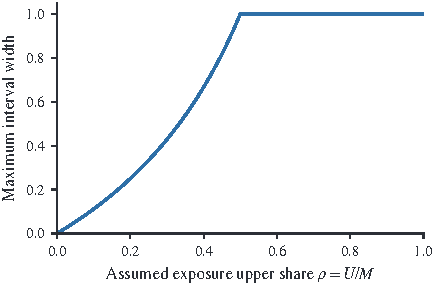
\includegraphics[width=0.52\textwidth]{figures/tmlrs_slr_novelty_bounds.pdf}
\caption{Parameterized sensitivity for the $M=\TTenM{}$ structurally
unresolved SLR-Bench items.  The curve shows the maximum interval width
over hypothetical binary correct fractions as the assumed exposure upper
share varies.  No model scores are used; width describes partial
identification, not sampling uncertainty.}
\label{tmlrs:fig:slr-novelty}
\end{figure}

\subsection{Overlapping Certificates}
\label{tmlrs:app:overlap}

For overlapping groups, let $A_{ji}=1$ when item $i$ belongs to certificate
group $G_j$.  The compatible exposure assignments solve
\[
\min/\max\ w^\top z
\quad\text{subject to}\quad
\ell\leq Az\leq u,\qquad z\in\{0,1\}^N.
\]
The toolkit function
\texttt{solve\_overlapping\_certificate\_bounds} solves this binary program
by mixed-integer linear programming for systems with at most 200 items.
Larger systems, or an explicit \texttt{lp} request, replace binary membership
by $z\in[0,1]^N$.  The resulting interval is an outer interval and is labeled
as such rather than being reported as attained by a binary assignment.

Each relaxed endpoint includes an independently checkable weak-duality
certificate.  For the lower endpoint, nonnegative
$(\alpha,\beta,\gamma)$ satisfying
\[
A^\top(\beta-\alpha)-\gamma\leq w
\]
certifies
\[
\ell^\top\beta-u^\top\alpha-\mathbf 1^\top\gamma
\leq \min w^\top z.
\]
The upper endpoint applies the same check to $-w$.  A separate verifier
checks dimensions, signs, feasibility, and the claimed objective within
$10^{-9}$.

The relaxation can be strict.  With three items and exact-one constraints on
$\{1,2\}$, $\{2,3\}$, and $\{1,3\}$, no binary assignment is feasible, while
$z=(1/2,1/2,1/2)$ satisfies the relaxation and gives interval
$[\TNineOddLower{},\TNineOddUpper{}]$.
Focused deterministic properties compare \TNineMilpCases{} random small
systems with exhaustive enumeration and independently verify
\TNineDualCases{} generated dual certificates, in addition to this odd-cycle
case and the existing disjoint-certificate regression tests.

\subsection{Falsification and Design Consequences}

The disjoint closed-form function still rejects overlapping certificate
groups, preserving its existing contract; the new solver handles those
systems explicitly.  Both interfaces reject incoherent bounds and
out-of-range indices.  An assignment checker directly falsifies a certificate
if observed identities violate its interval.

The proposition changes reporting and design in four ways: report
\([L,U]\), never code no-witness rows as novel; rerun witnesses after split
mutation; persist semantic IDs and category assignments for online
generators; and keep exposure bounds separate from behavioral estimands.

\section{Portable Toolkit Validation}
\label{app:assurance}

The versioned \texttt{semantic-audit-v1} command exposes Tensor Logic and
Occam adapters through one schema.  Required fields include source revisions
and hashes, observation contracts and semantic-unit adequacy rules,
train/evaluation identities, semantic IDs, witness types, completeness,
overlap denominators, behavioral metadata, and claim wording.  The validator
enforces that exact evidence has a Boolean decision, sound lower bounds
establish only positive overlap, unresolved evidence asserts neither overlap
nor novelty, and every current adapter declares its observable semantics.

\begin{table}[H]
\caption{Benchmark-level implementation assurance.  Residual risk is kept
separate from identification bounds; no row implies a quantified
implementation-error rate.}
\label{tab:assurance}
\centering
\scriptsize
\setlength{\tabcolsep}{2.5pt}
\resizebox{\textwidth}{!}{%
\begin{tabular}{L{0.72in}L{1.12in}L{1.12in}L{1.38in}L{1.32in}L{1.20in}}
\toprule
Case & Semantic-ID implementation & Source traceability &
Soundness and validation coverage & Known failure mode & Residual risk \\
\midrule
Internal finite rules &
Complete 20-output vector &
Frozen generator, split, stream, and checkpoint hashes &
Exhaustive finite-map census; paired-manifest and metric recomputation &
Applies only to the finite deterministic domain &
Low conditional risk; implementation error is not rate-bounded \\
Boolean tasks &
Signed-literal vector, active mask, or literal subset &
Pinned released generators and full stream manifests &
Combinatorial injectivity plus separate-code-path collision and replacement checks &
Exactness is limited to the three selected released task definitions &
Low within those definitions; transfer to conflicting definitions is
unsupported \\
CLUTRR &
Ordered target and three-edge relation tuple &
Frozen CLUTRR extraction, source groups, manifests, and artifact hashes &
Deterministic extraction; source-group disjointness; 11 post-training
integrity classes and separate-code-path metric recomputation &
Task~1, length three, and the frozen relation parser only &
Unquantified parser risk; low within the validated materialization \\
SLR-Bench &
Token identity plus restricted-fragment canonicalizer &
Pinned \texttt{v1-All} release and row-level train--test witnesses &
Each reported semantic pair has a proof-producing witness; positive and
negative normalizer tests &
Aggregates, negation, arithmetic, and unresolved disjunction are not decided &
Low false-positive risk for reported witnesses; unknown missed overlap \\
Tensor Logic &
Endpoint-path and ordered-relation-schema IDs &
Pinned repository and graph artifacts &
Exhaustive post-scrub path re-enumeration; adapter canaries and schema tests &
No checkpoint, per-query predictions, or training logs &
Exposure remains an interval; behavioral impact is unresolved \\
Occam Markov &
Exact transition-tensor ID with grouped-seed certificates &
Pinned repository and enumerated seed range &
75,093-signature census; bound checker and grouped-seed tests &
Order assignments are unpersisted; regression code is absent &
Interval retained for Markov tasks; regression scope remains unresolved \\
\bottomrule
\end{tabular}%
}
\end{table}

\paragraph{Validator independence dimensions.}
We use no unqualified independence claim.  A validator can differ from a
producer by implementation, code path, execution environment, operator, or
source specification.  ``Separate-code-path recomputation'' below means a
different analysis or checking routine consumes frozen producer artifacts.
``Isolated reproduction'' means a fresh process and dependency environment.
All validators remain in the same project and use the same frozen protocol;
we claim neither an independent human operator nor an independently authored
specification.

\begin{table}[H]
\caption{Producer--validator relationships for the major validated claims.
Shared dependencies limit the assurance each check supplies.}
\label{tab:validator-map}
\centering
\scriptsize
\setlength{\tabcolsep}{2.5pt}
\resizebox{\textwidth}{!}{%
\begin{tabular}{L{1.05in}L{1.28in}L{1.50in}L{1.45in}L{1.38in}}
\toprule
Claim & Producer & Validator & Distinct dimension & Shared dependency \\
\midrule
Internal exact-alias effect &
Training drivers and saved predictions &
Effect reconstruction from paired manifests and predictions &
Separate metric code path &
Same repository, protocol, artifacts, and operator \\
Boolean exposure and effect &
Stream materialization, training, and predictions &
Collision replacement checks and cluster-effect recomputation &
Separate checking and analysis paths &
Same released generators, protocol, repository, and operator \\
CLUTRR V4 effect &
32 training runs and prediction artifacts &
\texttt{train\_integrity.py} plus assignment and metric reconstruction &
Separate integrity and effect-analysis modules &
Same tensor caches, manifests, preregistration, repository, and operator \\
SLR 45.2\% lower bound &
Restricted-fragment parser and canonicalizer &
Row-level witness checks, positive canaries, and negative normalizer tests &
Separate witness and test paths &
Same normalization rules, source data, repository, and operator \\
Tensor Logic and Occam outputs &
Benchmark-specific adapters &
Common schema validator and two isolated reproductions &
Separate validator code; fresh process and environment &
Same adapter specification, pinned sources, repository, and operator \\
Certified interval &
Bound implementation &
Assignment checker and exhaustive finite cases &
Separate test path &
Same proposition, assumptions, repository, and operator \\
\bottomrule
\end{tabular}%
}
\end{table}

Eleven tests cover the three required canaries, schema rejection, and both
public adapters.  Two isolated \texttt{python3 -I} reproductions use no
third-party runtime package and produce byte-identical adapter outputs,
manifest, and checksums.  All portability checks pass; they validate the
toolkit and do not change the original breadth decision.

\section{Reproducibility Map}
\label{app:repro}

\begin{table}[H]
\caption{Claim-to-artifact map.  Paths are relative to the audit supplement
root supplied with the manuscript.  The public artifact repository is
\url{https://github.com/zihanzhou0725/semantic-novelty-audit-artifact}.}
\label{tab:repro-map}
\centering
\small
\begin{tabular}{L{1.3in}L{4.4in}}
\toprule
Claim or artifact & Reproduction source \\
\midrule
Internal exact audit (historical p1) &
\url{analysis/quality-enhancement-v1/p1/results.json} and frozen paired manifests \\
SLR lower bound &
\url{artifacts/slr_overlap_results.json}, token witnesses, and semantic witnesses \\
SLR identification decision (historical p2) &
\url{analysis/quality-enhancement-v1/p2/identification_report.json} \\
Boolean coverage &
\url{protocols/boolean-behavioral-v1/split_manifest.json} \\
Boolean behavior &
\url{analysis/boolean-behavioral-v1/results.json} and paired episode CSV \\
Prospective external audits (historical p3) &
\url{analysis/quality-enhancement-v1/p3/} and candidate manifest \\
CLUTRR V3 pilot and diagnosis &
\url{results/v3/}, \url{design/v3_variance_results.json}, and frozen protocols \\
CLUTRR V4 confirmation &
\url{results/v4/}, \url{design/v4_design_manifest.json}, frozen protocols, and
\url{analysis/external-behavior-v4/cluster-sensitivity-v1/} \\
Portable toolkit (historical p4) &
\url{analysis/quality-enhancement-v1/p4/} and \url{toolkit/semantic_audit/} \\
Certified interval (historical p5) &
\url{analysis/quality-enhancement-v1/p5/} and executable bounds tests \\
Integrity &
protocol/full-matrix validators and frozen checksums \\
\bottomrule
\end{tabular}
\end{table}

\begin{table}[H]
\caption{Strengthening analyses.  Paths are relative to the audit supplement
root; the directory prefix \texttt{analysis/tmlr-strengthening-v1/} applies
to the five result paths.}
\label{tab:repro-strengthening}
\centering
\small
\begin{tabular}{L{1.3in}L{4.4in}}
\toprule
Claim or artifact & Reproduction source \\
\midrule
CLUTRR heterogeneity (T2) &
\url{t2_clutrr_heterogeneity/summary.json};
inputs in \url{analysis/external-behavior-v4/effect-analysis-v1/} \\
Internal heterogeneity (T3a) &
\url{t3_internal_heterogeneity/summary_heterogeneity.json};
\url{analysis/quality-enhancement-v1/p1/function_effects.csv} \\
Semantic versus decoy (T6) &
\url{t6_semantic_vs_surface/summary.json};
\url{protocols/tmlr-strengthening-v1/t6_semantic_vs_surface/protocol.json};
compact predictions in \url{artifacts/tmlr_t6_run_outputs/} \\
Overlapping bounds (T9) &
\url{t9_overlapping_certificates/property_tests_summary.json};
\url{toolkit/semantic_audit/bounds.py} \\
Parameterized sensitivity (T10) &
\url{t10_novelty_bounds/summary.json};
\url{artifacts/slr_overlap_results.json} (structural counts only) \\
\bottomrule
\end{tabular}
\end{table}

From the manuscript directory, \texttt{make reproduce-paper}
regenerates T2, T3a, T6, T9, and T10 from retained evidence, copies their
macros and figures, regenerates the overview, and runs \texttt{latexmk}.
Set \texttt{PYTHON} to an environment with the supplement dependencies
and \texttt{AUDIT\_ROOT} to the audit supplement directory if it is not
in the default sibling layout.  No model training is required.

\section{Additional Limitations}

The SLR proof covers only a restricted positive fragment and does not decide
semantic equivalence for the entire Prolog language.  The per-item SLR model
artifact cannot establish the paper-model effect because its aggregate does
not match either published table.  The internal protocol contrast changes
more than duplicate membership.  The Boolean intervention covers one model
configuration and released generators whose Sparse Disjunction, Sparse
Parity, and Threshold definitions conflict with parts of the paper.  The
three-seed directional criterion was preregistered, but between-seed uncertainty is
coarse; the hierarchical and Student-$t$ intervals are therefore both shown.
The original prospective breadth criterion remains unmet because only one frozen
candidate is complete and neither supplies credible behavioral evidence.
The later CLUTRR study supplies an independent public behavioral
confirmation but covers one relation length, architecture, exposure dose, and
training budget.  The certified interval is tight only relative to the
supplied certificate system; adding sound constraints can narrow it.  None of
these synthetic findings determines contamination prevalence in
natural-language benchmarks.


\end{document}
